\chapter{Cosmic rays}
\label{ch:cosmic-rays}


\section{A brief history of cosmic-ray research}

% Observed effects of cosmic rays without special instruments, e.g. aurora.

The effects of low-energy solar cosmic rays were already seen in ancient times. This was in the form of the aurora borealis and aurora australis. Several ancient written recordings of the phenomenon \cite{stephenson2004aurora} have been found, moreover, many folk tales about this phenomenon exist. The cause of the aurorae was not known then. In 1600 Gilbert created a terrela, a sphere with a magnetic field resembling that of the Earth \cite{gilbert1893terrella}. In 1896 Birkeland \cite{lilensten2012terrella} showed that electron beams fired at a terrela were bent along the field lines to form circular regions around the magnetic poles like the aurora. The aurora appears to be caused by disturbances in the magnetosphere of the Earth. The disturbances are generally caused by solar winds. Magnetic reconnection occurs and causes charged particles to be accelerated into the atmosphere \cite{angelopoulos2008reconnection}. There the particles will excite and ionize oxygen and nitrogen atoms. When these de-excite or recombine the auroral colors are produced. An example of the aurora can be seen in \cref{fig:aurora}.

\begin{figure}
    \centering
    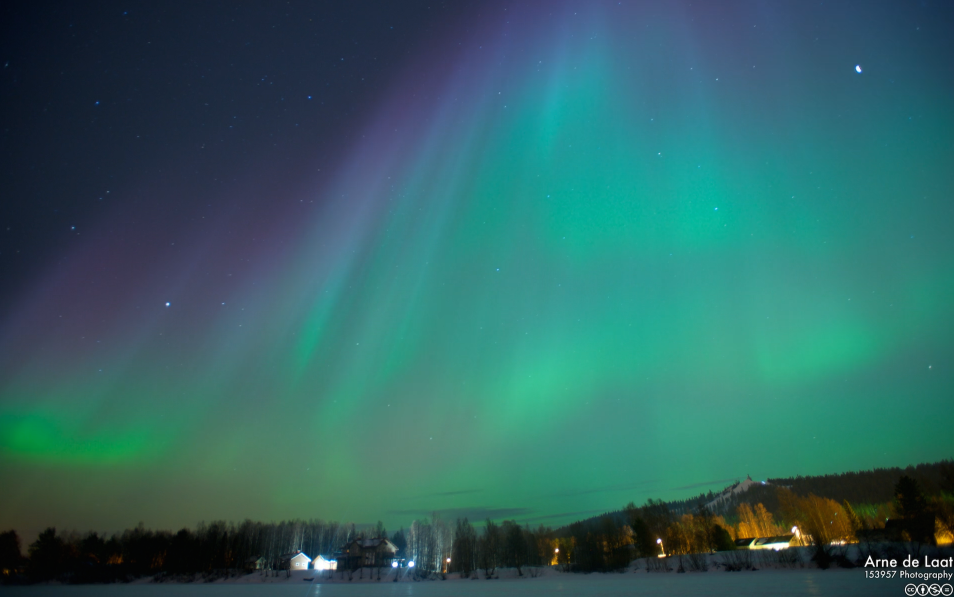
\includegraphics[width=0.6\textwidth]{plots/cosmic-rays/aurora.png}
    \caption{Aurora borealis as seen in Rovanemi, Finland on 17 March 2015, St. Patricks day. The large aurora activity on that day was due to a G4 geomagnetic storm on the sun two days earlier. The interactions between the incoming electrons and the atoms in the atmosphere creates the fluorescence. In this case the red and green colors are caused by different excitation energies in the atomic oxygen.}
    \label{fig:aurora}
\end{figure}

% Briefly talk about the discovery of the background radiation (caused by cosmic rays) and the discovery of where they come from (i.e. not radiation from Earth).
% How it was discovered that cosmic rays were charged particles.
% How this all lead to cosmic-ray research and the discovery of extensive air showers.

\subsection{Discovery of cosmic rays}

In 1785 the effects of cosmic rays were detected by de Coulomb \cite{fokkema2012hisparc} with an electroscope. An electroscope measures the amount of electrical charge in a test object. De Coulomb saw it unexpectedly discharge in the air, even though it was properly insulated. In 1895 the discovery of X-rays and their capability to ionize air \cite{flakus1981radiation} presented a good candidate for why the electroscope discharged. However, a source of the X-rays had not yet been identified. In 1896 Becquerel discovered the existence of radioactivity \cite{badash1965becquerel}. he also found that the radiation from radioactive material could cause an electroscope to discharge. Further experiments with the electroscopes were performed to assertain the source of the ionizing radiation. Experiments went over seas, underwater \cite{pacini2011sea}, underground, and far above ground \cite{angelis2013history}, but no conclusive evidence for cosmic rays was found until Hess performed balloon flights in 1911 and 1912 which accurately determined the amount of radiation at various altitudes. It showed a clear increase at very high altitudes, indicating an extra-terrestial source for the radiation. Clay \cite{clay1928latitude} found that the intensity of the ionization depended on latitude. This latitudinal dependency could be caused by the magnatic field of the Earth. Being affected by magnetic fields indicates that the particles were charged particles \cite{compton1932charged}. The indepent discovery of extensive air showers (EAS) in the atmosphere by Auger (1939) \cite{auger1939eas} and Rossi (1934) \cite{rossi1934eas} ignited the cosmic-ray research field.


\section{Cosmic ray source and their journey}

Cosmic rays are very energetic particles moving through space. Some impact Earth's atmosphere causing cascades of particles. Most commonly cosmic rays are protons, heavier atomic nuclei are the next most common component. A small fraction of the cosmic ray flux are electrons and gamma rays. Anti-particle cosmic rays have also been observed.

% What (some of) the expected origins/sources of cosmic-rays are.
The cosmic rays reaching Earth have energies anywhere from \SIrange{e9}{e21}{\eV}. Objects in space where these particles are accelerated have not yet been unequivocally identified. A strong contributing suspect are Supernova Remnants (SNR). A SNR consists of shockwaves of particles ejected by a supernova explosion. A shockwave occurs when particles are moving faster than the local speed of sound. SNRs pass through the Interstellar Medium (ISM), the region between stars in the galaxy. Here the shock picks up particles and possibly accelerates them, taking energy out of the shockwave \cite{helder2009snr}. The Fermi Large Area Telescope (LAT) discovered evidence for \Pgpz-decay in SNRs \cite{ackermann2013snr}, which is an indicator for energetic protons. Neutral pions can be created in energetic proton-proton collisions. Models predict that SNRs can contribute a significant fraction of the cosmic-ray flux up to \SI{e15}{\eV} \cite{cardillo2015snr}. Models predicting the creation of the very high energetic cosmic rays (VHECR) in Active Galactic Nuclei (AGN) and pulsars exist, but evidence for these processes has not yet been discovered.

% The acceleration mechanisms that come into play.

\subsection{Cosmic voyage}

% What the cosmic rays encounter along the way.
Cosmic rays do not travel through a perfect vacuum. The ISM is filled with particles, radiation and magnetic fields. The interstellar matter consists mainly of atomic hydrogen (\SI{70.4}{\percent} by mass), but also of helium (\SI{28.1}{\percent}), the rest (\SI{1.5}{\percent}) are heavier metals. With an average density of \SI{1}{particle\per\centi\meter\cubed} or \SI{2.7e-24}{\gram\per\centi\meter\cubed} \cite{ferriere2001ism}. Though the ISM is far from homogenous, it will be assumed for a moment. Imagine a proton travelling the diameter of the Milky Way (\SI{40}{\kilo\parsec}, or \SI{1.2e23}{\cm}) before reaching Earth. This particle will have passed through a column depth of \SI{0.324}{\gram\centi\meter\squared}. This is very small relative to the thickness of Earth's atmosphere. The thickness of the Earth's atmosphere and the mean free path of cosmic rays in it will be discussed in \cref{sec:cr:eas}.

% Explantation for the GZK cutoff/limit.
Radiation fields can in some cases affect the cosmic rays. With energies above \SI{5e19}{\eV} proton cosmic rays can interact with photons from the cosmic microwave background (CMB). In these collisions pions can be produced (via \PDelta) and the primary cosmic ray may lose up to \SI{20}{\percent} of its energy. The density of the CMB photons is \SI{550}{\per\centi\meter\cubed}. With a cross section of approximately $\sigma_{\Pproton \gamma_{CMB}} = \SI{2e-28}{\centi\meter\squared}$ at these high proton energies. This limits the possible distance from which these particles can originate and still reach Earth without undergoing this interaction. If a source of extremely energetic cosmic rays is close enough the particles may make it without undergoing these energy loss interactions. Above \SI{2e20}{\eV} the cosmic-ray flux is supressed by over a factor of 100. This upper limit of cosmic-ray energy is known as the Greisen Zatsepin Kuzmin (GZK) limit \cite{zatsepin1966gzk,greisen1966gzk}.

% How the direction of cosmic rays no longer points to their origin, gyro radius.
Cosmic rays do not simply travel in a straight line from their source to Earth. Moving charged particles are affects by magnetic fields. The Lorentz force may change the direction of the particle. The strength of this depends on the angle between the direction of motion and magnetic field lines. The deflection is strongest when the field is perpendicular to the direction of motion. The strength of all magnetic fields in the universe is not known. The overal field strength and distribution of large scale random fields for the Milky Way are being determined from experiments. The average magnetic field strength is \SI{0.6 \pm .2}{\nano\tesla} \cite{jansson2010magnetic}. The radius of curvature for relativistic particles traveling through a magnetic field is called the Larmor radius (or gyro radius). This is given by
%
\begin{equation}
    R = \SI{108}{\kilo\parsec}
        \frac{E_{\si{\exa\eV}}}{Z B_{\si{\nano\tesla}}}
\end{equation}
%
where $R$ is the radius of curvature, $Z$ the atomic number of the particle, which is equal to the charge because atomic cosmic rays are fully ionised, $B$ is the magnetic field strength, and $E$ the energy of the particle. In \cref{fig:gyroradius} the gyroradius of a proton cosmic ray is shown for various energies of the cosmic ray and various strengths of the magnetic field \cite{grigat2011anisotropy}.

\begin{figure}
    \centering
    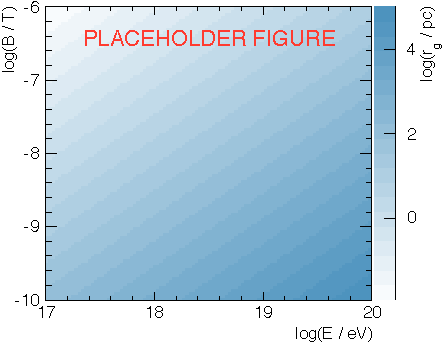
\includegraphics[width=0.6\textwidth]
                    {plots/cosmic-rays/gyroradius}
    \caption{The gyro radius of primary proton cosmic rays as a function of their energy for different magnetic field strengths. The amount of deflection greatly depends on the actual average magnetic field strength in the Milky Way, which is not precisely known. Indicated are sizes of important astronomical objects.}
    \label{fig:gyroradius}
\end{figure}

% This leads to isotropy at low energies, and possibly anisotropy at very high energies.
If the energy of a cosmic ray is low enough it may be captured by a galaxy. This can happen if the gyro radius is significantly smaller than the object. For the Milky Way this transition is around \SIrange{e16}{e18}{\eV}. For particles at and below these energies the paths though the ISM will not be straight. The deflections will cause the directions of the particles at Earth to be randomised, i.e. isotropically distributed. At low enough energies the particles are also affected by the solar wind, a cause for possible anisotropy. Above these energies, the particle paths will be straighter. Unless it encounters strong local fluctuations in the magnetic field. For cosmic rays of high enough energy anisotropy may be expected if there are clearly defined sources on the sky.

Heavy particles have smaller gyro radii and are therefore more easily contained. Consequently, heavy particles may be accelerated to higher energies at their source, being contained until accelerated to high enough energies to escape. The cosmic rays of energies above this transition can escape from the Milky Way. Similarly cosmic rays in other galaxies can escape if they have enough energy. From observations the average magnetic field strength in other visible spiral galaxies is on average \SI{.9 \pm .3}{\nano\tesla} \cite{jansson2010magnetic}. In the intergalactic medium (IGM) the particle density is approximately \SIrange{0.1}{0.25}{\per\meter\cubed} \cite{copi1995igm}. The expected average magnetic field strength in the IGM is \SI{< e-4}{\nano\tesla} \cite{kronberg1994igm}.

Knowledge about the exact distribution, strength, direction, and changes over time of the magnetic fields in the universe are not at out disposal. This makes it difficult/impossible to fully reconstruct the path of arriving cosmic rays.


\subsection{Final destination}

% Explain what cosmic rays are seen at Earth, as observed by experiments.
% How various models explain the spectrum; different compositions, galactic, extra-galactic.
At Earth cosmic rays arrive from all directions. On average the flux as a function of different energies is constant. In \cref{fig:spectrum} the measured differential flux of cosmic rays at the top of the atmosphere is shown. At low energies the flux varies over time due to solar modulation. The solar cycle of \SI{11}{\year} affects the flux in this energy region of cosmic rays. The top axis shows the equivalent center of mass collision energies. This can be used to relate the energy in the cosmic ray collision to the collision energies reported for particle colliders on Earth. At the 'end' of the spectrum, around \SI{e20}{\eV} the spectrum steepens and seems to end. No cosmic rays above $E = \SI{e21}{\eV}$ have yet been detected. The reasons for this is probably the GZK limit explained earlier. But may also be explained by the lack of sources being able to produce such highly energetic particles.

\begin{figure}
    \centering
    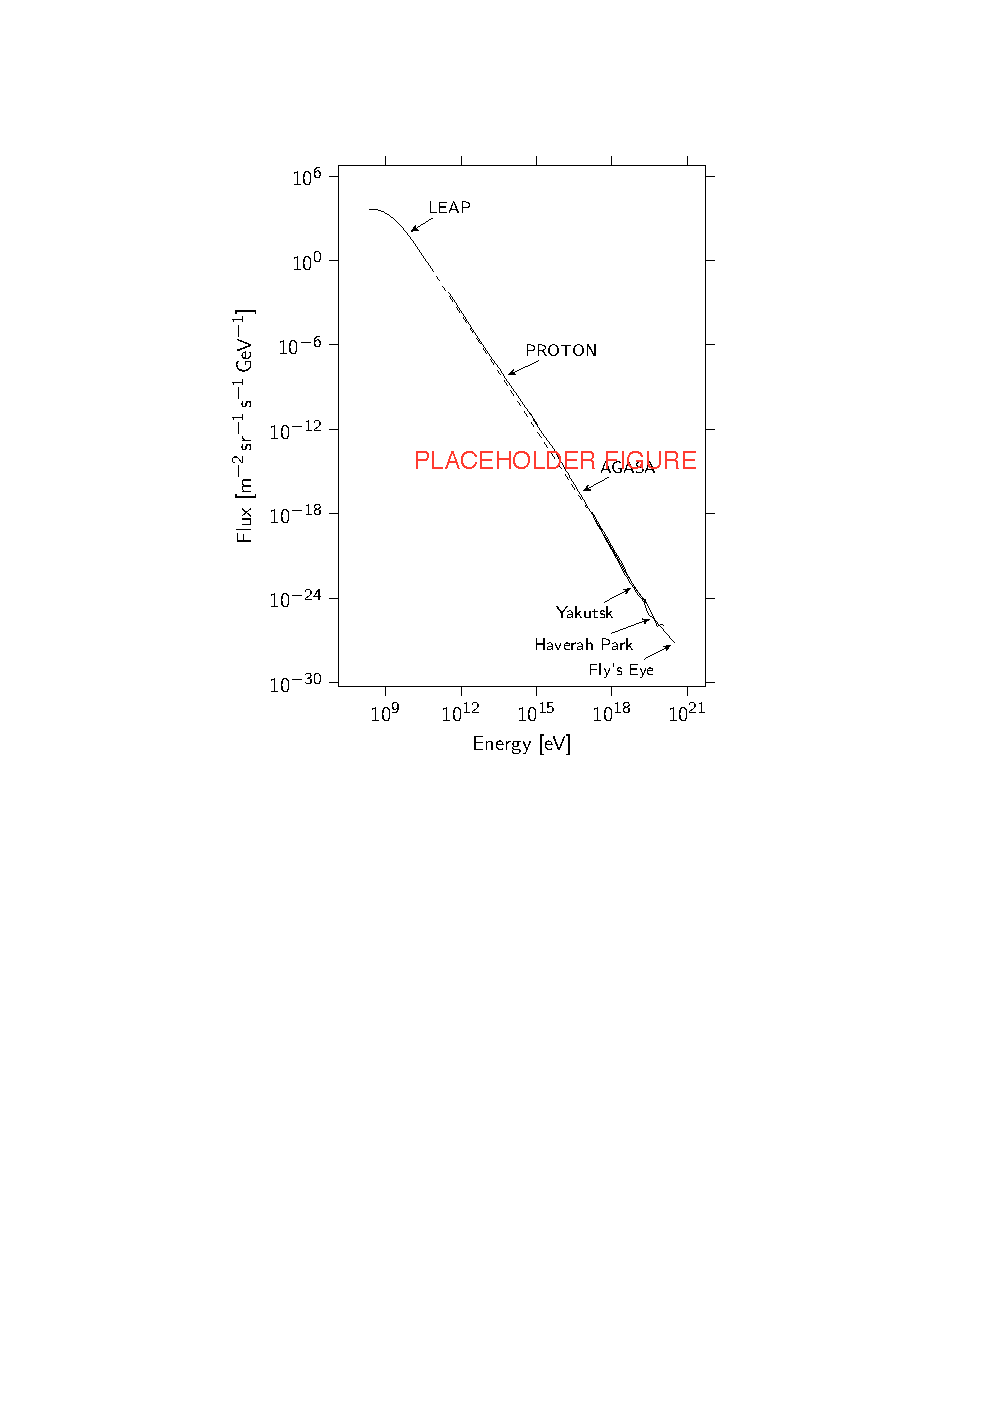
\includegraphics[width=0.6\textwidth]{plots/cosmic-rays/spectrum.pdf}
    \caption{Differential flux of primary cosmic rays versus the kinetic energy per particle. The spectral index of the spectrum is approximately $\gamma = 2.7$. Around $E = \SI{e15}{\eV}$ is the transition from directly (lower energies) to indirectly (higher energies) detected cosmic rays. At low energies the flux is indicated by a band because it changes over time due to solar modulation. Less low energy cosmic rays are observed during high solar activity. [Todo:] Equivalent center of mass collision energies as top x-axis. Marked are the achieved p-p (and p-Pb) collision energies in colliders. The transition from Galactic and extra-Galactic is determined from the expected gyro radii in the Milky Way. Also shown are likely source contributions at some energies (SNR).}
    \label{fig:spectrum}
\end{figure}


% Explain the possibilities of direct detection of cosmic rays: Low energy, balloon, space.
Cosmic rays can be detected in multiple ways. Either by detecting them directly or indirectly. In order to directly detect cosmic rays the detector needs to be above or high in the Earth's atmosphere (above \SI{25}{\kilo\meter}). This is typically done by balloon-borne experiments or space-based missions. Due to the low flux of high energy cosmic rays these methods are mainly aimed at the lower energies ($E < \SI{e15}{\eV}$). For cosmic rays of higher energies the particle cascades they create in the atmosphere are used. These cascades can be detected from the ground. The physics and characteristics of these particle showers are discussed further in \cref{sec:cr:eas}.

\subsection{Direct detection}

% What is learned from direct detection experiments: Composition, Solar modulation, van Allen belt, heliosphere, particle-antiparticle fraction, isotropy.
Being able to directly detect the particle has the advantage of easy particle identification. The main downside is the flux of cosmic-rays decreases steeply when looking at higher-energy cosmic rays. Ideally the detector has a large detection area and a very long exposure time. Unfortunately a detector that has to be flown to the top of the atmosphere or in space can only be so big before it costs too much to launch. Balloon experiments are often short runs where the balloon carrying the detector stays up for about a week. The JACEE \cite{asakimori1998jacee} and RUNJOB \cite{hareyama2011runjob} experiments flew multiple times. Each experiment reached a total fly time of \SI{60}{\day}. Notable space-based missions are PAMELA \cite{adriani2014pamela}, in orbit on the Resurs DK1 sattelite since 2006, and the AMS-02 \cite{casaus2014ams} experiment attached to the International Space Station (ISS) since 2011. These space-based experiments have been operating for many years. The measurements provide good resolution on the composition of cosmic rays at energies upto the knee \cite{amenomori2008knee}. At the knee the spectral index of the cosmic ray flux changes from $\gamma = 2.7$ to 3.1.

These experiments are able to measure the modulation of the low-energy cosmic-ray flux due to the solar activity. During high solar activity (many sunspots) the flux of galactic cosmic rays at Earth is reduced \cite{adriani2013modulation}. This is the reason for the band seen at low flux in \cref{fig:spectrum}. Also the ratio of normal and anti-particles has been determined. For electrons about \SI{15}{\percent} of the particles around \SI{e11}{\eV} are positrons \cite{aguilar2013positrons}. The \APproton/\Pproton fraction settles around \SI{2e-2}{\percent} for energies above \SI{e10}{\eV} \cite{kappl2015antiproton}. No anisotropy has been found in the arrival directions of \APelectron\Pelectron cosmic rays detected by these experiments \cite{panico2015isotropy}.

Together these direct detection experiments provide a very detailed picture of the low energy cosmic-ray spectrum. The per-nucleus spectrum of such experiments is shown in \cref{fig:PDG_28_1_fluxes_per_nucleus}.

\begin{figure}
    \centering
    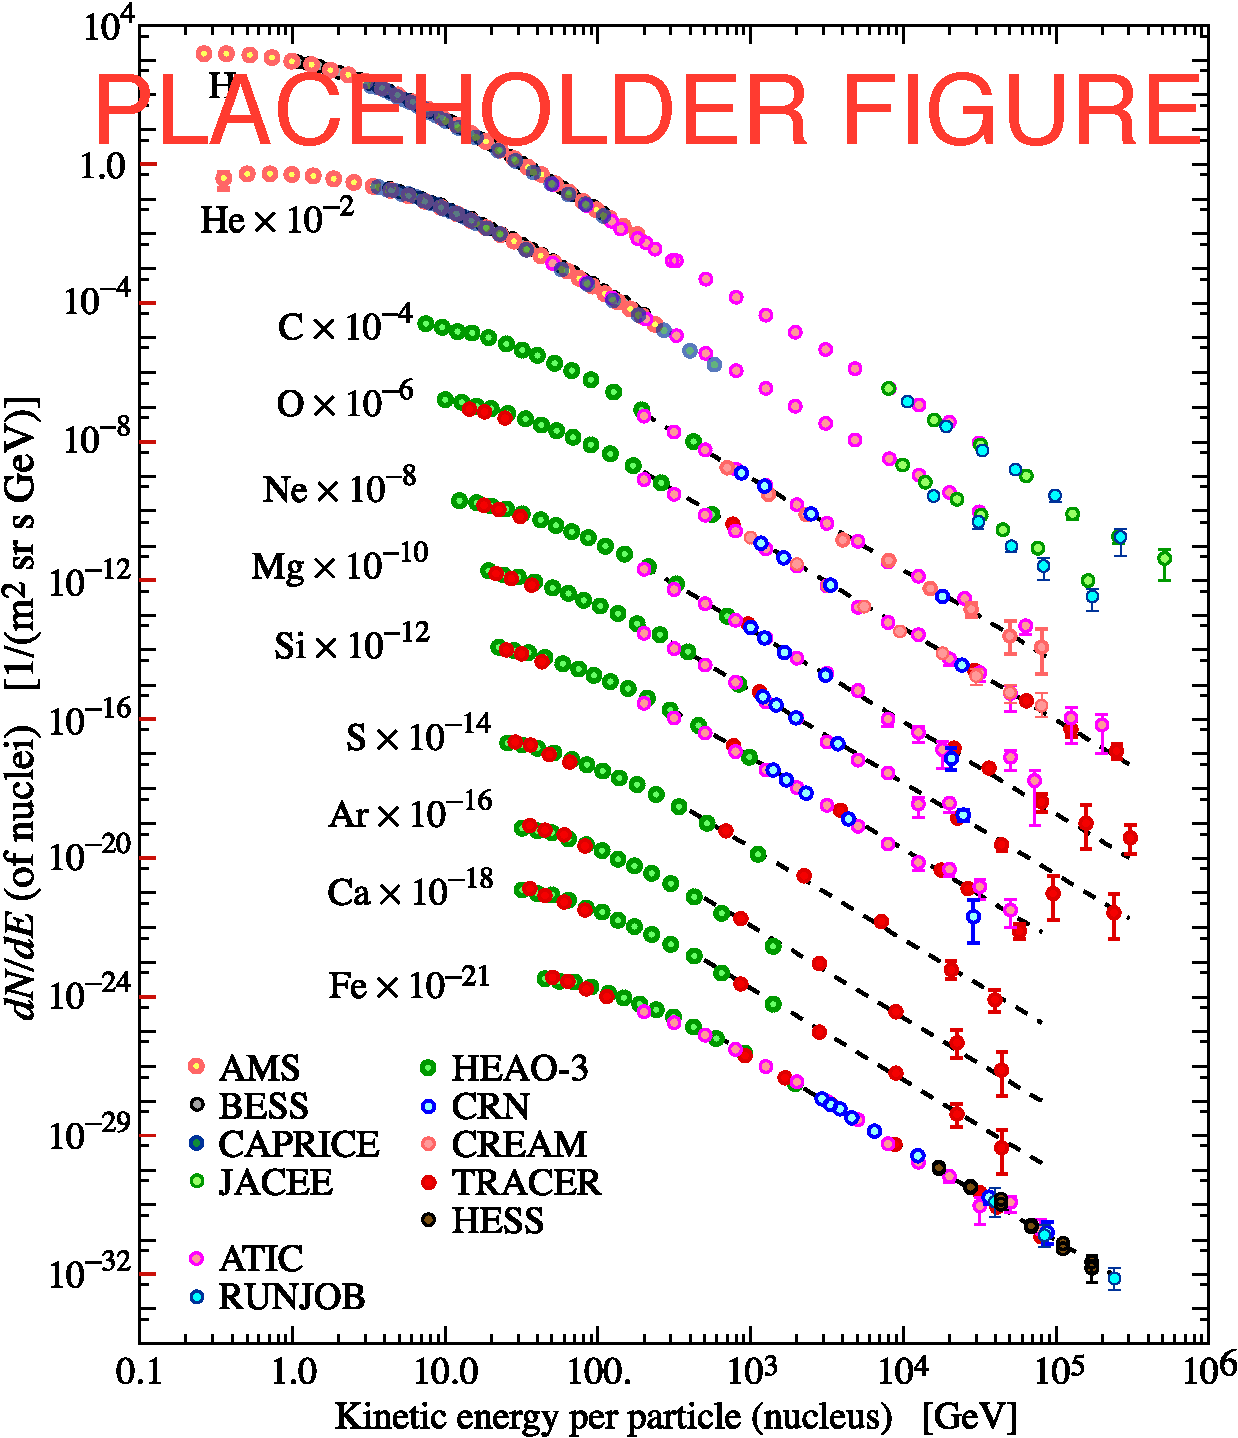
\includegraphics[width=0.6\textwidth]
                    {plots/cosmic-rays/PDG_28_1_fluxes_per_nucleus.pdf}
    \caption{Decomposed differential flux of primary cosmic rays. Balloon and space experiments directly detecting cosmic-rays provide composition data for the cosmic-rays.}
    \label{fig:PDG_28_1_fluxes_per_nucleus}
\end{figure}

The longest running space-based cosmic-ray experiments are the Voyager spacecrafts. The Pioneer probes, also carrying a cosmic-ray detector, were launched about 4 years earlier, but contact with them was lost over a decade ago. The Voyager spacecrafts were launched in 1977 to use the planetary alignment to accelerate with several gravity assists \cite{stone1977voyager}. In August 2011 Voyager I seems to have reached the heliopause of the solar system, at \SI{121}{\astronomicalunit} distance to the Sun. Here the detection rate of particles caused by the solar wind (>\SI{5e8}{\eV}) decreased steeply and the rate of cosmic-ray particles from outside the solar system (>\SI{7e10}{\eV}) increased significantly \cite{stone2013voyager}. The measurements from Voyager I are shown in \cref{fig:voyager_heliosphere}. Cosmic rays of these energies are thought to originate from supernovae in this galaxy.

\begin{figure}
    \centering
    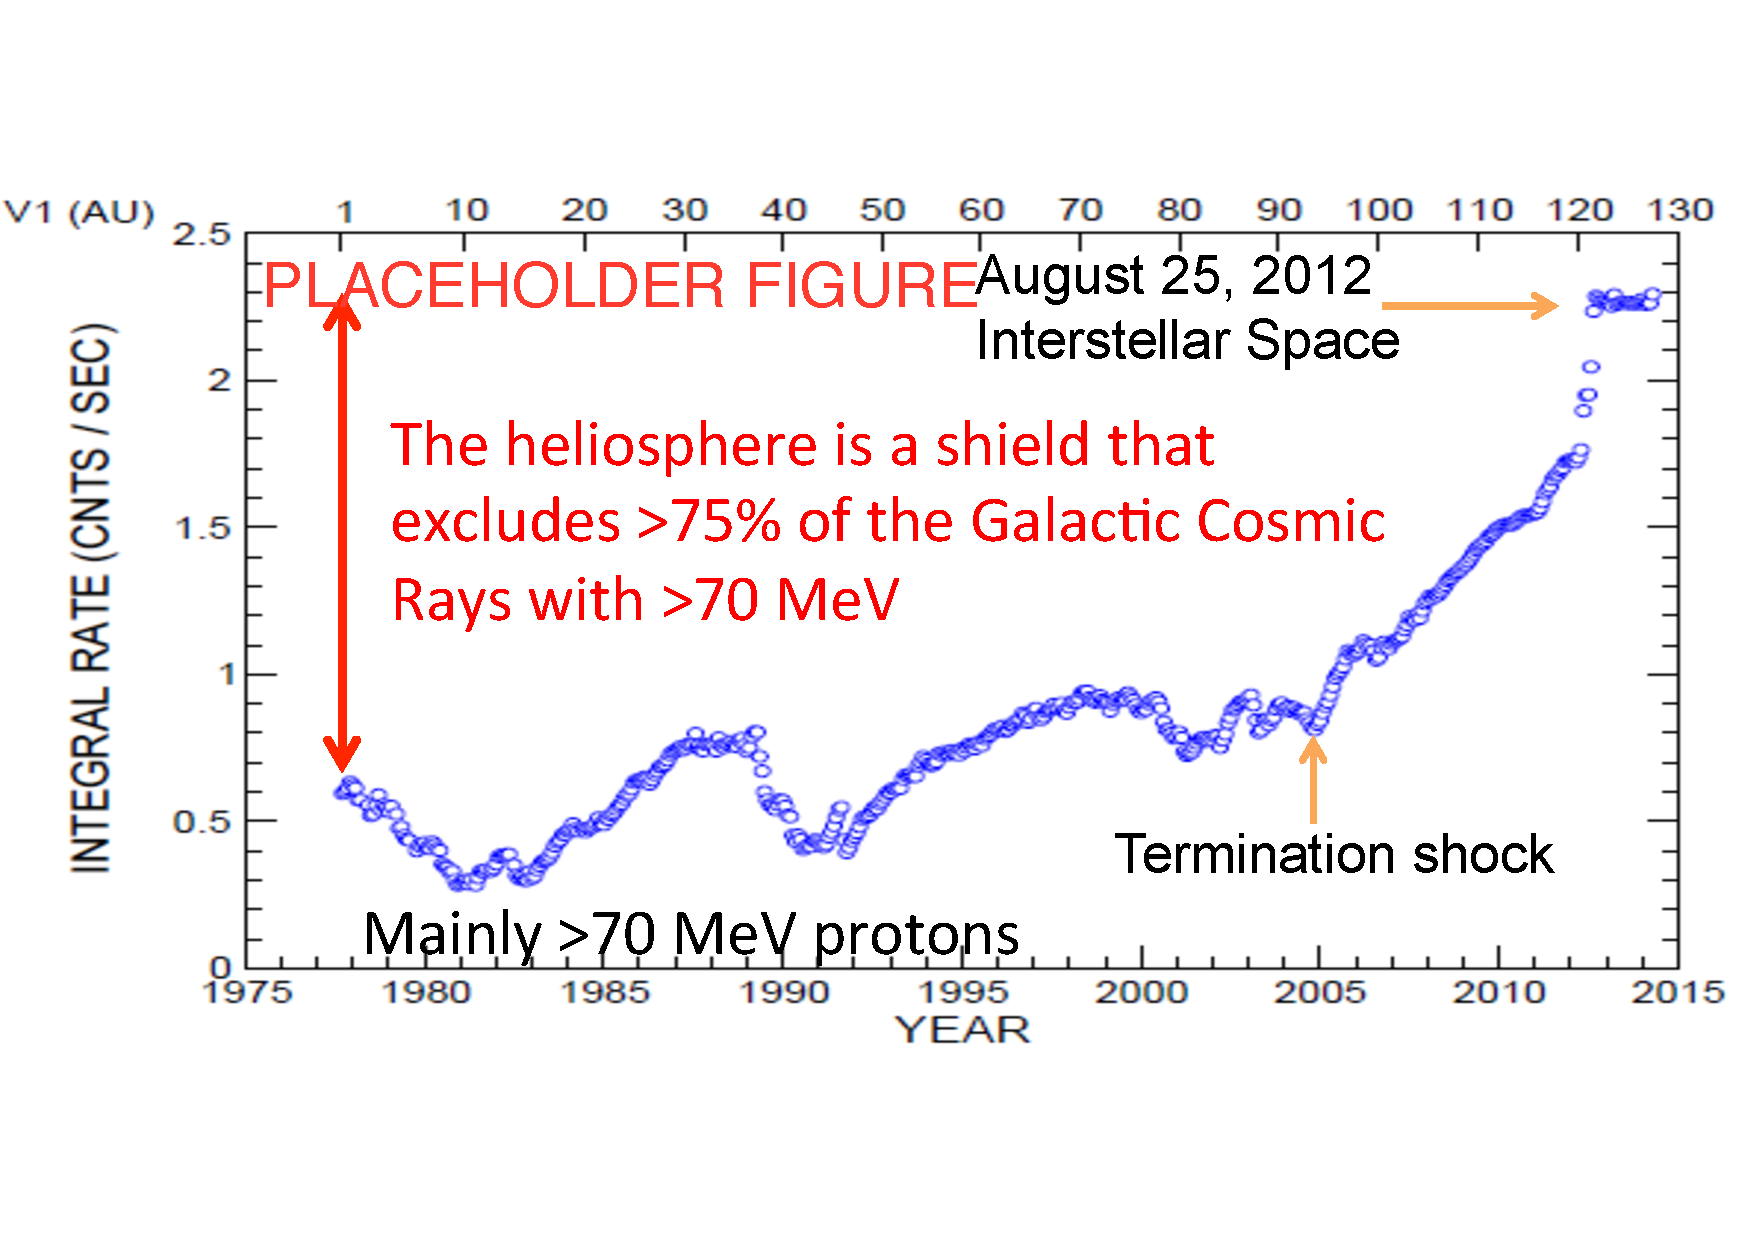
\includegraphics[width=0.6\textwidth]
                    {plots/cosmic-rays/voyager_heliosphere}
    \caption{Extrasolar cosmic ray rate by Voyager 1, stone2015]
Timeline of the cosmic ray rate measured by the Voyager 1 spaceprobe. The rate started to increase when it passed the termination shock. After passing the heliopause the rate has stabilized at 4 times the rate inside the heliosphere. This is a measure of the cosmic ray rate unaffected by solar winds.}
    \label{fig:voyager_heliosphere}
\end{figure}


\subsection{Indirect detection}

% How high-energy cosmic rays may hold information about anisotropies and possible sources (hot spot).

Currently the two biggest ground-based cosmic-ray experiments are the Pierre Auger Observatory (Auger) \cite{abraham2004auger} in Argentina and the Telescope Array (TA) \cite{abu-zayyad2012ta} in Utah. Both use particle detectors and fluorescence detectors overlooking the particle detector area. Auger has been expanded with radio detectors. Because of their size (\SI{3000}{\kilo\meter\squared} and \SI{700}{\kilo\meter\squared} respectively). and separation between the particle detectors (\SI{1.5}{\kilo\meter} and \SI{1.2}{\kilo\meter}) these experiments are looking for cosmic-rays at the highest energies. The minimum energy threshold for both experiments, ignoring the smaller low energy extensions, is above \SI{e18}{\eV}. Several cosmic-rays of $E > \SI{e20}{\eV}$ have been detected by both epxeriments, settings limits on the high-energy cosmic ray spectrum and probing the GZK limit. At these high energies possibilities for anisotropy exist. In \cref{fig:skymap_ta_auger} a combined sky map of cosmic rays detected by both experiments shows a dipole moment deviations from isotropy \cite{abbasi2015combined}. When considering only primaries with energies above $\SI{57e18}{\eV}$ the TA sees a slight preference for cosmic rays from a region on the sky, shown in \cref{fig:hotspot_ta} \cite{ta2014hotspot}. However, with a significance of $3.4 \sigma$ more data is needed to verify the excess.

\begin{figure}
    \centering
    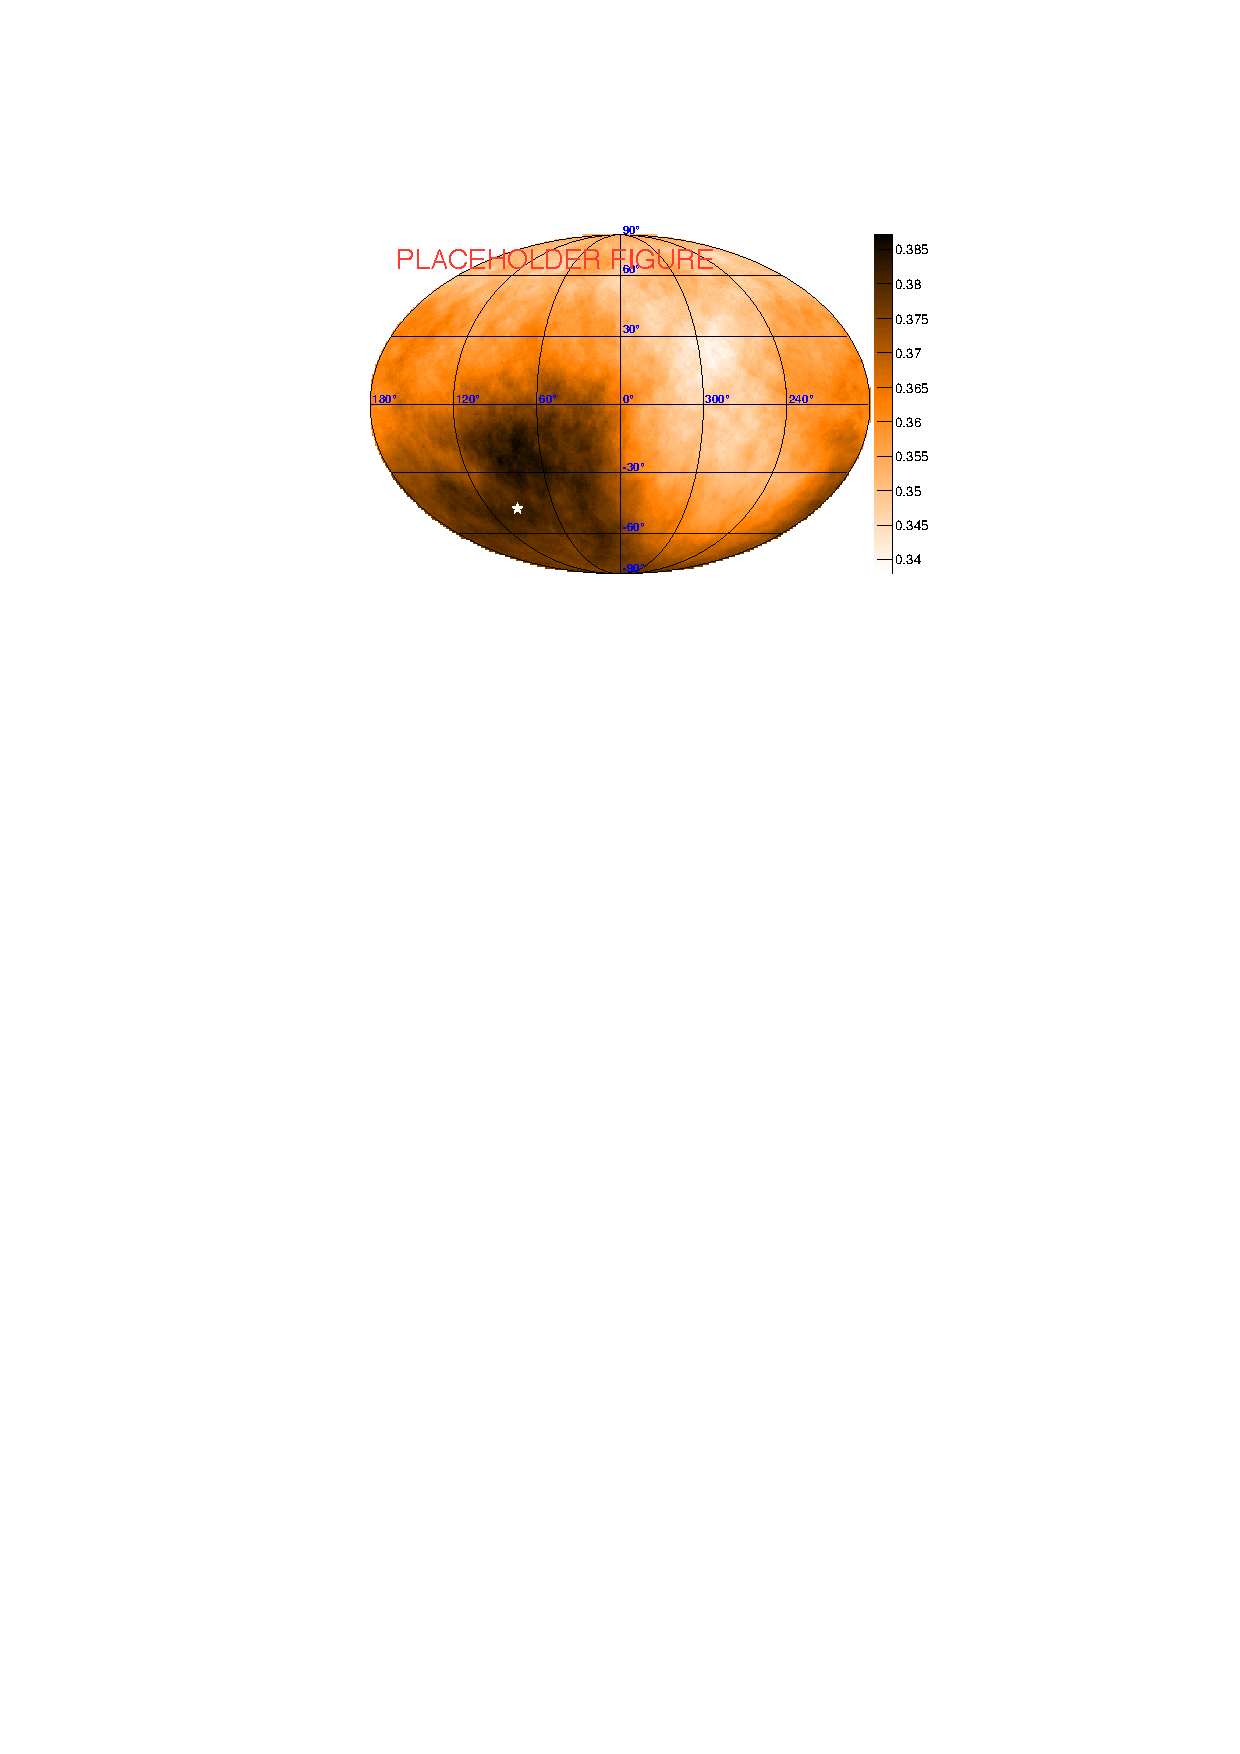
\includegraphics[width=0.6\textwidth]
                    {plots/cosmic-rays/skymap_ta_auger}
    \caption{Anisotropy measurement for cosmic rays of $E > \SI{e19}{\eV}$ by the combined Pierre Auger Observatory and Telescope Array data. The overlapping regions are used to correct for sensitivity differences between the experiments. Only a dipole moment is seen, higher multipoles do not deviate from the expected fluctuations of an isotropic flux at \SI{99}{\percent} confidence level. The color scale units are in \si{\per\kilo\meter\squared\per\year\per\steradian}}
    \label{fig:skymap_ta_auger}
\end{figure}

\begin{figure}
    \centering
    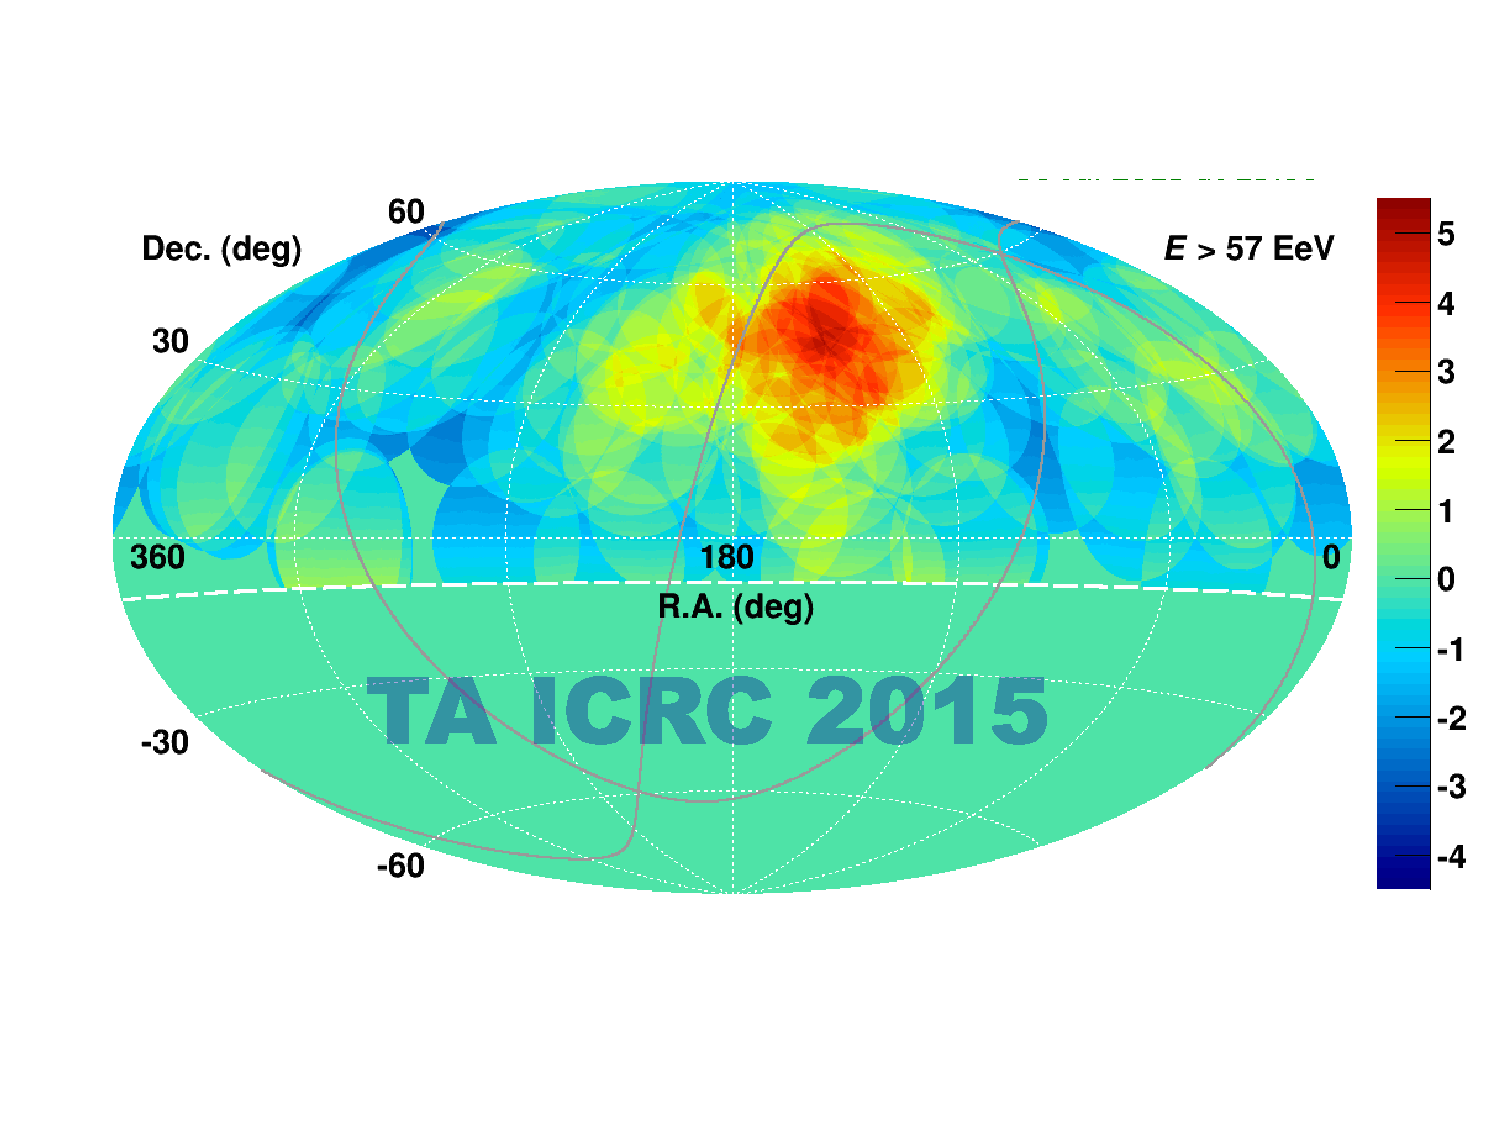
\includegraphics[width=0.6\textwidth]
                    {plots/cosmic-rays/hotspot_ta}
    \caption{Hot spot by TA on mollweide plot, abasi2015]
Anisotropy significance plot for the Telescope Array data for primary cosmic rays of $E > \SI{57e18}{\eV}$. Here a hot spot with a significance of $3.4 \sigma$ is observed. This may indicate a source, but more data is required for a more definite conclusion.}
    \label{fig:hotspot_ta}
\end{figure}

% Highlight some of the features of the high energy spectrum, and that there is some composition information known (light-heavy) but no exact fractions.
In \cref{fig:PDG_28_8_all_particle_spectrum} the height of the spectrum is compressed by scaling the data by $E^{2.6}$. This way certain features are more easily seen. For instance the changes in the steepness of the power law (knees and ancles) are more visible. Composition measurements are less specific for indirect measurements. They do provide an indication for the overall lightness (mostly protons) or heaviness (more biased towards iron) of the composition. It appears that beyond $E = \SI{e18}{\eV}$ the composition becomes heavier \cite{abbasi2015combined}. However, the model predictions upon which these measurements depend are not yet perfect. Improvements to the experiments are planned to increase the exposure and improve the sensitivity to the composition.

\begin{figure}
    \centering
    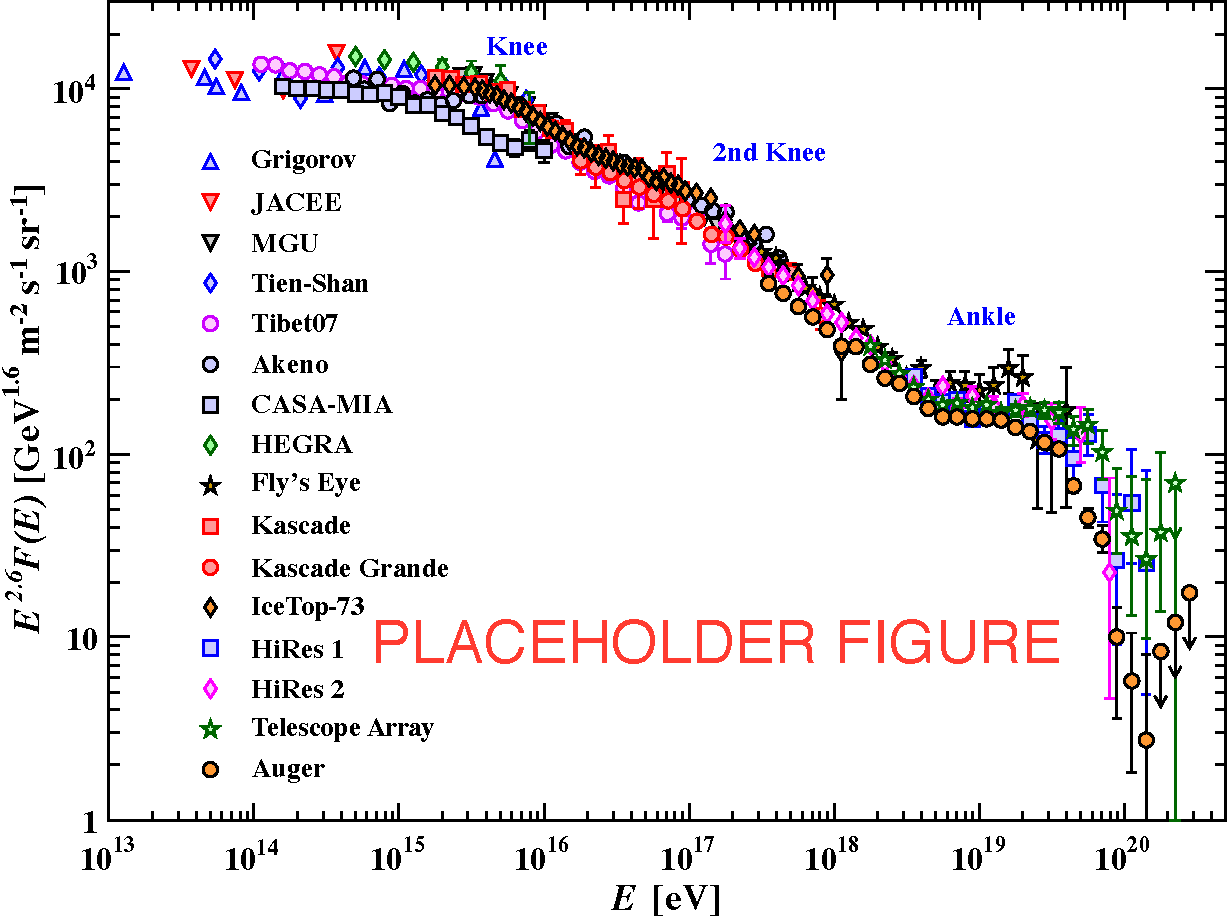
\includegraphics[width=0.6\textwidth]
                    {plots/cosmic-rays/PDG_28_8_all_particle_spectrum}
    \caption{Detailed spectrum at high energies]
The differential flux of cosmic rays multiplied by $E^{2.6}$. This representation of the latest data from cosmic-ray experiments reveals more structure in the spectrum. Little data is available for the highest energy cosmic rays, but limits are set on the maximum rates. The composition of cosmic rays at these energies is not yet known.}
    \label{fig:PDG_28_8_all_particle_spectrum}
\end{figure}


\section{Extensive air showers}
\label{sec:cr:eas}

% Typical hadronic interactions of (hadronic) cosmic rays entering the atmosphere.
% The cross section of such interactions, as known from colliders and cosmic ray experiments.
% Colliders not yet upto highest energies, and different type of interactions.
The first interaction target of incoming cosmic rays are the atoms in the upper atmosphere. The upper atmosphere consists mainly of nitrogen (\SI{78.1}{\percent}), oxygen (\SI{21.0}{\percent}), and argon (\SI{0.9}{\percent}) \cite{noaa1976atmosphere}. Unfortunately collider experiments rarely use these nuclei as collision material. So the exact cross section of interactions between cosmic-rays (any ion from protons to iron) and air is not known at high energies.

Particle colliders like HERA \cite{abramowicz1999hera}, RHIC \cite{harrison2003rhic}, and SPS \cite{bozzo1984sps} have been able to produce collisions center mass energies of several hunderds \si{\GeV}, equivalent to cosmic rays of \SI{e14}{\eV} colliding with a fixed target.

The collider data has been essential for tuning models simulating the interaction in the particle cascades. Using extrapolations models can simulate the expected showers for cosmic-rays of the highest energies. The expected accuracy of the extrapolations becomes less the further they are from the collider data. These colliders provide important data about the hadron production processes in air showers, the cross-sections of the collisions, the multiplicity of secondary high-energy particles and the ratio of neutral to charged particles \cite{pierog2008lhc}.

Fermilab's Tevatron was capable of proton collisions with center of mass energies of \SI{1.8}{\TeV} \cite{abe1994tevatron}, equivalent to collisions of cosmic protons with \SI{2e15}{\eV} against a fixed target. This is approximately the lower energy limit for the \kascade experiment \cite{antoni2003kascade}. However, \kascade's upper limit was \SI{e17}{\eV}. The LHC is in an interesting energy range; \SI{7}{\TeV} and now upgraded to \SI{14}{\TeV}, equivalent to \SI{2e16}{\eV} and \SI{e17}{\eV} cosmic-ray energies respectively. These are the first time that we have access in colliders to collision energies above the knee in the cosmic-ray spectrum. This also covers the entire energy range of the \kascade experiment. This is not true for the high energy \kascade-Grande extension of \kascade \cite{apel2010kascadegrande}. The hadronic interaction models from before the LHC did not properly predict the new LHC data at energies beyond the Tevatron. The EPOS \cite{pierog2015epos} and QGSJETII \cite{ostapchenko2013qgsjetii} models have been updated using LHC data from the \SI{7}{\TeV} run. This should provide more accurate results for higher energies. Shower simulations used for this thesis were performed before data from the LHC run at \SI{14}{\TeV} had been incorporated into models.

The TOTEM \cite{antchev2010totem,antchev2011totem} and LHCf \cite{adriani2008lhcf} experiments at the LHC are placed at the forward regions of the CMS and ATLAS interaction points respectively. These provide the most interessing data for cosmic-ray physics because the interesting products of collisions are those with high pseudorapidity. The LHC runs with p-p collisions most of the time, short periods are run with heavy ions collisions (p-Pb and Pb-Pb). However, for cosmic-ray physics collisions with low-mass ions (oxygen) that are commonly part of the interactions of EAS would be more interesting. Collision data of such interactions would greatly benefit cosmic-ray research.

From p-p collisions the p-Air cross sections can be extrapolated using the Glauber formalism \cite{glauber1955crosssections,abbasi2015crosssection}. In \cref{fig:pair_crosssection} the proton-Air inelastic collision (i.e. new particles are created) cross section is shown. Measurements by various experiments (points) and predictions by models (lines) are given. At higher energies the models deviate significantly from each other.

\begin{figure}
    \centering
    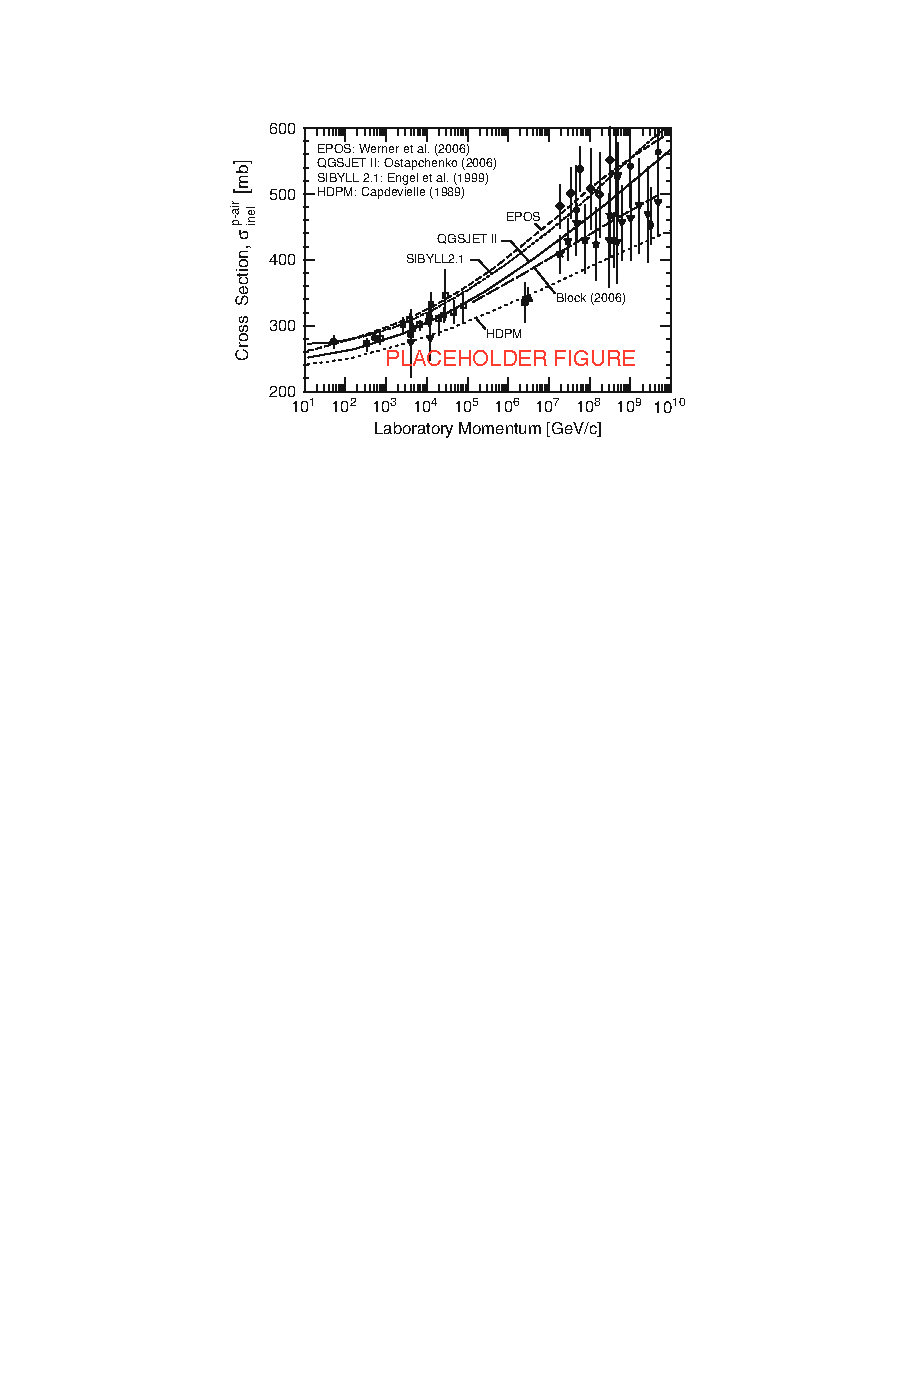
\includegraphics[width=0.6\textwidth]
                    {plots/cosmic-rays/pair_crosssection}
    \caption{The measured inelastic proton-air cross section determined from cosmic ray measurements of the first interaction altitude. As the energy of the particles increases, so does the cross section. The measurements are within the predicted values from proton-proton cross sections measured in colliders when corrected with Glauber theory.}
    \label{fig:pair_crosssection}
\end{figure}

% Provide the model of the thickness of the atmosphere as a function of the height (as used in CORSIKA).

The density gradient of the atmosphere is the next important factor. The atoms in the atmosphere are the potential targets for the incomming cosmic ray. Earth's atmosphere has been extensively measured and parameterized. As the density increases, so does the probability of a collision. The common way to describe the atmosphere is by giving the column depth, i.e. the amount of material a particle will have passed since it entered Earth's atmosphere. The atmospheric depth is given by
%
\begin{equation}
    X = \int \rho(h) \diff h
\end{equation}
%
where $X$ is the atmospheric depth, $\rho$ is the density of the atmosphere as a function of height above ground ($h$). In \cref{fig:atmospheric_depth} the atmospheric depth is shown versus the height above sea level. At sea level the atmospheric depth is approximately \SI{1e3}{\gram\per\meter\squared}. This is the column depth for vertically incoming particles. However, cosmic rays also enter the atmosphere at angles. In this case the path through the atmosphere is longer by approximately $\cos^{-1} \theta$. The resulting column depth is called the slant depth.

\begin{figure}
    \centering
    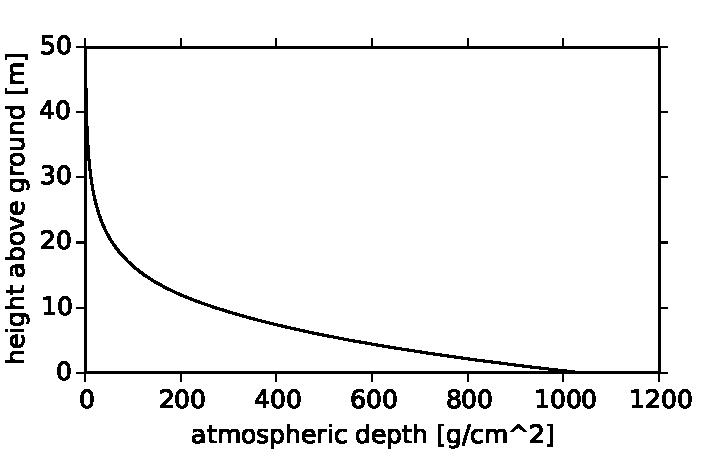
\includegraphics[width=0.6\textwidth]
                    {plots/cosmic-rays/atmospheric_depth}
    \caption{The atmospheric depth as a function of altitude above ground for the U.S. standard atmosphere \cite{heck2013corsika}. The air becomes thinner higher above the ground.}
    \label{fig:atmospheric_depth}
\end{figure}

% The combination of cross section and atmospheric depth gives a distribution for the likely first interaction altitudes.
Monte Carlo simulations using the above described model of the atmosphere and the interaction model QGSJETII-04 give insight in the distribution of the first interaction altitude. In \cref{fig:first_interaction_altitude} the first interaction altitude distribution is shown for vertically incomming proton primaries of $E = \SI{16}{\eV}$. On average the primaries interact around \SI{22}{\kilo\meter} above ground where the distribution has a FWHM ~\SI{15}{\kilo\meter}. Cosmic rays of higher energy have a higher mean interaction altitude, since the cross section increases with energy, as was shown in \cref{fig:pair_crosssection}.

\begin{figure}
    \centering
    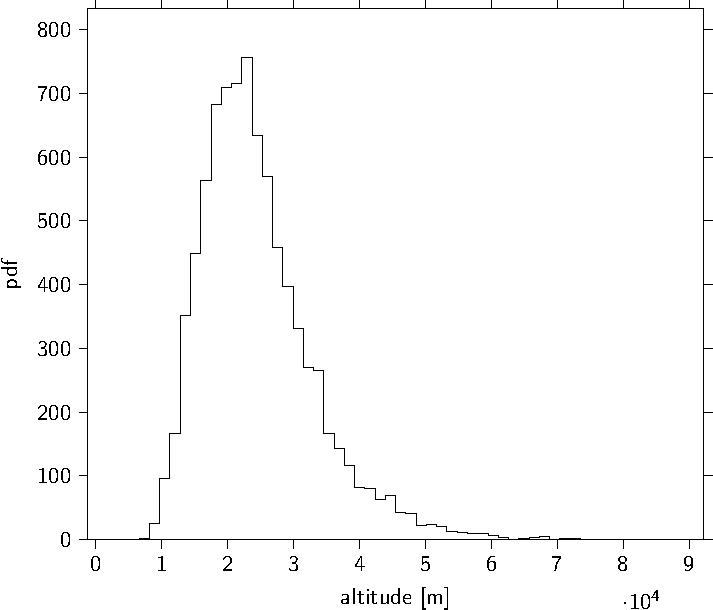
\includegraphics[width=0.6\textwidth]
                    {plots/cosmic-rays/first_interaction_altitude}
    \caption{Distribution of first interaction altitudes for primary proton cosmic-rays of $E = \SI{16}{\eV}$. From the cross sections a mean free path can be calculated for cosmic rays entering the atmosphere. \cite{heck2013corsika}}
    \label{fig:first_interaction_altitude}
\end{figure}

For inclined cosmic rays higher column depths are reached at higher altitudes, increasing the mean height of the first interaction.

% Explain that these hadronic interactions can produce many secondaries (multiplicty).

The hadronic interaction between the primary hadron and the nuclei produce a number of new particles. The number of generated particles is energy dependend \cite{grieder2010eas}. The mean number of generated charged particles in a proton-proton collision is shown in \cref{fig:multiplicity}. In a shower multiple hadronic interactions occur, the initial has the highest energy. The interactions generate new particles until the energy of the colliding particles falls below the threshold required to produce a pion. They may still undergo interactions at lower energies, but those are of no interest to the shower development.

\begin{figure}
    \centering
    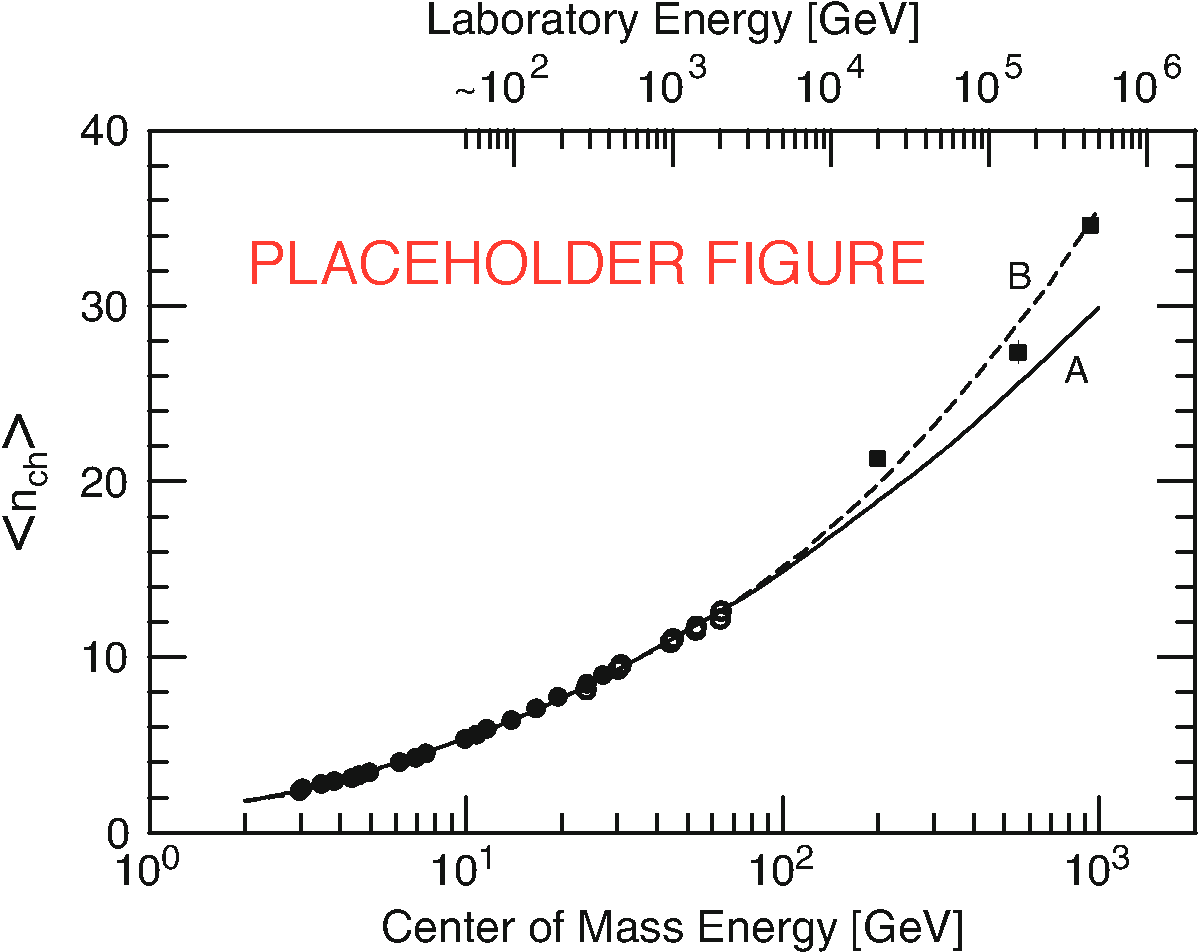
\includegraphics[width=0.6\textwidth]
                    {plots/cosmic-rays/multiplicity}
    \caption{Average charged secondary particle multiplicty in p-p collisions as a function of the collision energy. The multiplicty increases with the energy of the collision. Results from collider data is shown along with models that try to predict the behavior at higher energies. Predictions vary widely from model to model.}
    \label{fig:multiplicity}
\end{figure}

% Explain what particles are produced and what happens to them.
The most commonly produced particles in the hadronic interactions are light mesons. Neutral and charged pions are most commonly generated. In these interactions conservation laws apply. This means the convervation of baryon and lepton number, energy, momentum, angular momentum, and charge. Each (anti-)quark has a baryon number of $(-)\frac{1}{3}$. Mesons consist of a quark and anti-quark, so have a baryon number of 0. So mesons can 'freely' be added to the output of the interaction. As long as enough energy is available to produce the particles. A typical collision can be
%
\begin{equation}
    \HepProcess{\Pproton + \Pproton \to \Pproton + \Pproton + i \Ppiplus + i \Ppiminus + j \Ppizero},
\end{equation}
%
Here $i$ and $j$ can be any positive integer. These reactions are not fully elastic, because new particles are created. However, the incident particle, or parts of it, generally survive and still carry a significant fraction of the energy.

% Explain how energy is transferred into the leptonic part of the shower.
% Particle creation with energy transfer from hadronic to EM
The neutral pions quickly decay (a mean life time of $\tau = \SI{8.4e-8}{\ns}$) via the electromagnetic force into two gamma rays (\SI{98.8}{\percent} of the time) \cite{olive2014pdg}.
%
\begin{equation}
    \HepProcess{\Ppizero \to \Pphoton + \Pphoton}.
\end{equation}
%
Here the baryon number is conserved because leptons, neutrinos, and bosons have a baryon number of 0, equal to that of a meson. The gammas will initiate new electromagnetic cascades. Note that quoted mean lifetimes are for the particle at rest. Given the relativistic nature of the particles in showers, due to the high energies, the mean lifetime are longer in the lab/Earth frame.

The charged pions decay a bit slower ($\tau = \SI{26}{\ns}$) into muons with same charge, and a (anti) muon neutrino \cite{olive2014pdg}.
%
\begin{equation}
    \HepProcess{\Ppiplus \to \APmuon + \Pnum},
    \HepProcess{\Ppiminus \to \Pmuon + \APnum}.
\end{equation}
%
The branching ratio for this process is \SI{99.99}{\percent}, the second most probable decay produces an electron and (anti) electron neutrino.
%
\begin{equation}
    \HepProcess{\Ppiplus \to \APelectron + \Pnue},
    \HepProcess{\Ppiminus \to \Pelectron + \APnue}.
\end{equation}

The mean lifetime of the muon is relatively long with $\tau = \SI{2197}{\ns}$ \cite{duclos1973muon}. The muons can easily reach ground if they have enough energy because of time dilation and length contraction. Some muons do decay before reaching ground in which case the \Pmuon (\APmuon) produces a electron (positron) and positron neutrino (electron neutrino),
%
\begin{equation}
    \HepProcess{\Pmuon \to \Pelectron + \APnue + \Pnum}, \\
    \HepProcess{\APmuon \to \Ppositron + \Pnue + \APnum}.
\end{equation}

In \cref{fig:schematic_shower} a schematic representation of the hadronic interction is seen. After the first interaction many new particles are created. The leading particle (the surviving part of the incident particle) continues towards the ground with a significant part of the energy. It will undergo further interactions, but with lower energy, and thus lower multiplicity.

The dominant interaction for the high energy photons created by neutral pion decay is pair production. The photons must have more energy then the rest mass of the two produced particles, i.e. \SI{1022e6}{\eV} for an electron postitron pair.
%
\begin{equation}
    \HepProcess{\Pgamma \to \Pelectron + \Ppositron}.
\end{equation}

Below this energy Compton scattering begins to dominate. In Compton scattering the photon recoils of another particle, transfering energy to the other particle.

% Explain Heitler model for EM shower.
Electrons and positrons in the cascade will mainly lose energy via Coulomb bremsstrahlung. In this process the electrons will emit photons when passing close to the nucleus of particles where they are affected by the electric fields of the charges. The mean free path of this process is of the same order as that for the pair production. So on average after each radiation length (mean free path) the photons will undergo pair production while the electrons produce new photons via bremsstrahlung. The number of particles doubles at each stage and the energy is divided over the particles. This simple way of describing the electromagnetic cascade is called the Heitler model \cite{matthews2005heitler}.

\begin{figure}
    \centering
    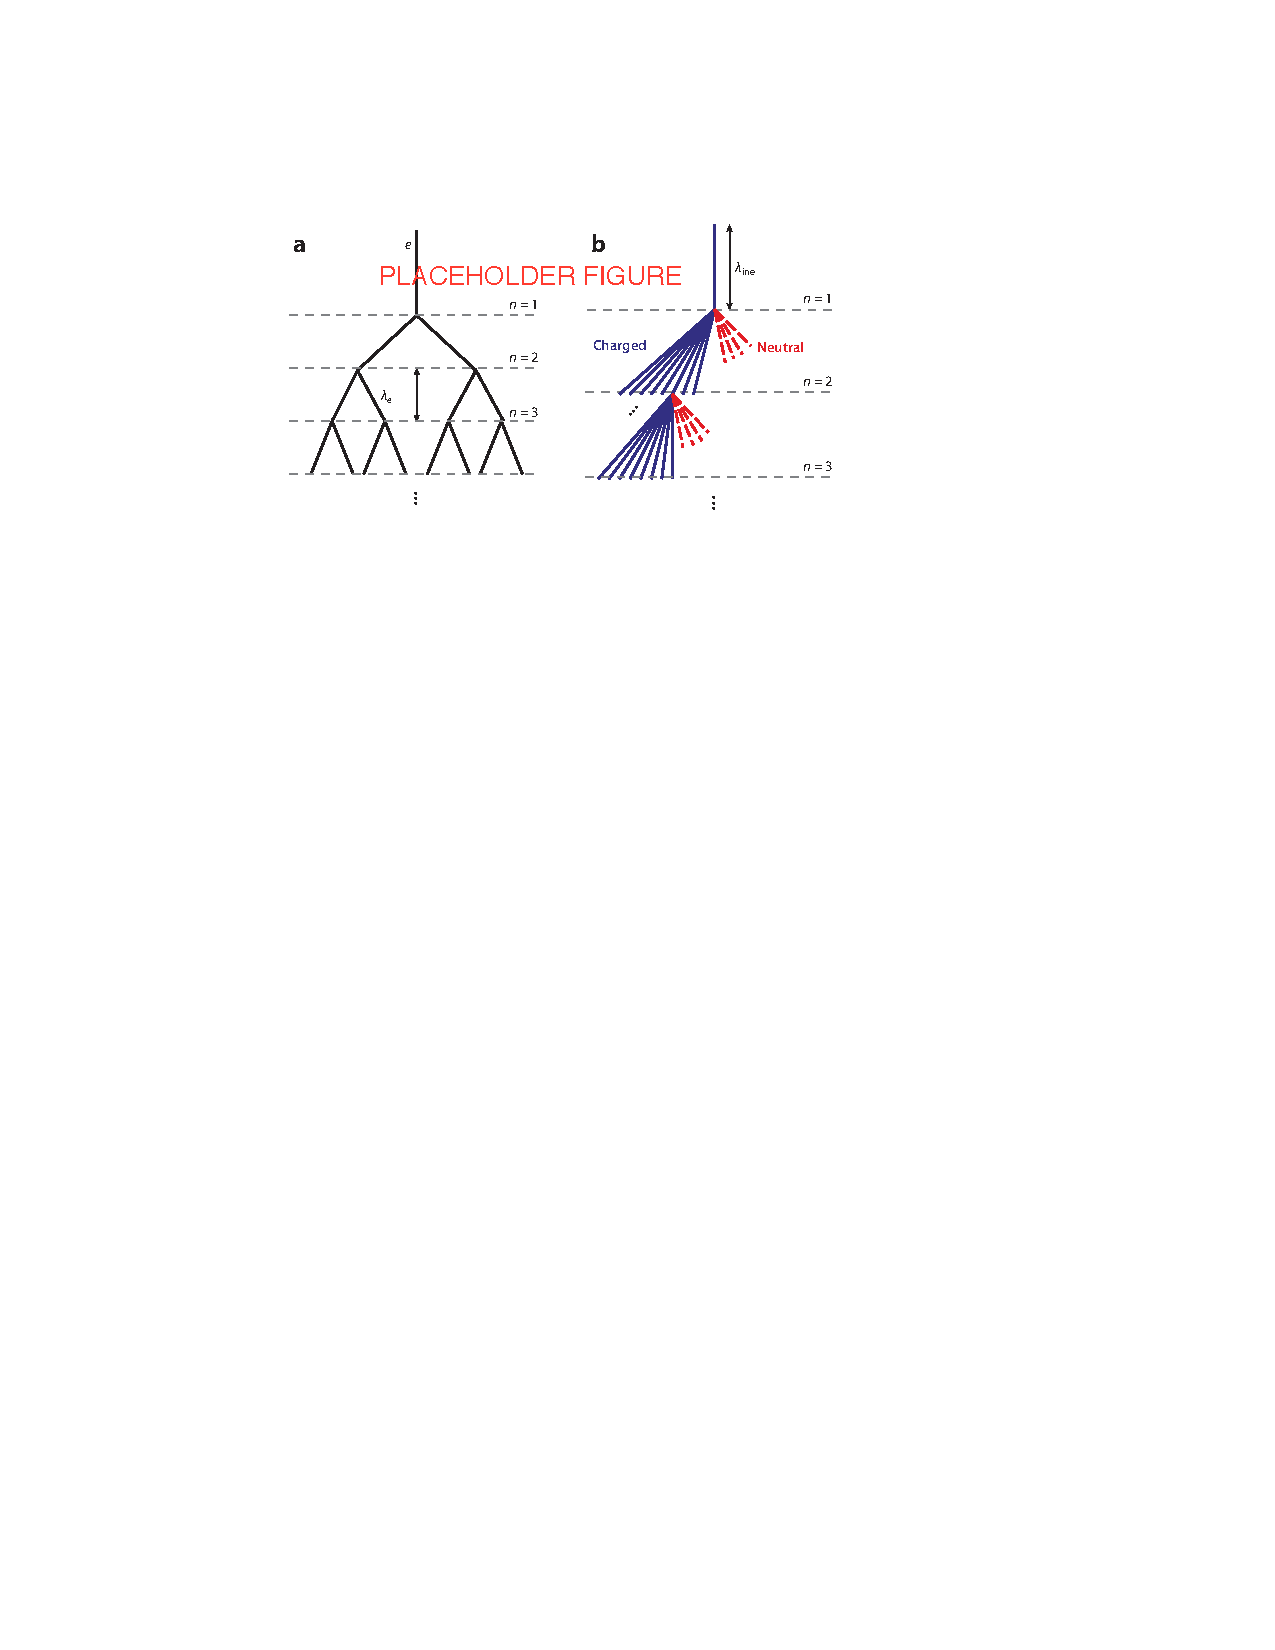
\includegraphics[width=0.6\textwidth]
                    {plots/cosmic-rays/schematic_shower}
    \caption{Simple representation of the hadronic and electromagnetic cascades in an air shower. The high multiplicity causes many new charged and neutral particles to be created. The subsequent hadronic interactions are at lower energies and thus, on average, lower multiplicty. After ~6 interaction lengths the shower has reached ground level and most energy will have gone to the electromagnetic shower. For the electromagnetic cascade start when neutral pions or muons decay into gammas or electrons. Gamma's undergo pair creation and electrons (and positrons) emit gammas due to bremsstrahlung. At each radiation length the number of particles doubled, as long as enough energy is available. \cite{engel2011eas}}
    \label{fig:schematic_shower}
\end{figure}

A full air shower initiated by an incoming hadron will consist of an hadronic component with many electromagnetic subcascades. In the hadronic cascade many pions are produced at different stages. These decay to the muons and gammas. The gammas, and to some extent muons, produce electrons and initiate the electromagnetic cascades.


\subsection{Other observables}
\label{sec:other_observables}

The charged particles reaching ground level are often used to detect the air showers. However, other observables are also created in the shower \cite{grieder2010eas}. The motion of the shower electrons through Earths magnetic field causes them to be slightly deflected, with the positrons being deflected in the opposite direction. In this process radio pulses are created, which can be detected by antennae. Cherenkov radiation is emitted as the fast charged particles move through the atmosphere. The angle of the Cherenkov cone changes with the energy of the shower particles and the height in the atmosphere. Since Cherenkov radiation is emitted along the entire length of the shower information about the development of the shower can be probed. Fluorescence caused by the ionization and excitation of the air causes fluorescence to be emitted along the entire track of the shower. This can also be used to observe the development of the shower from different sides. The fluorescence and Cherenkov radiation is not very bright. Detectors wishing to detect those signals can only operate when there is little background light. That means only at night, no moon, no clouds, no dust in the air, and not to much light polution. These requirements make the duty cycle of these detectors less than \SI{20}{\percent} \cite{abraham2004auger}.


\subsection{Longitudinal}

% This results in a longitudinal profile.
% Particle decay and absorption cause reduction in number of shower particles.
The balance between new particle creation and particle absorption changed as the average energy per particle changes during shower development. When the particles have a enough energy particle production dominates. As energy is spread thin among many particles the absorption will be come more important. Also the decay processed change the balance of hadrons, leptons and gammas. In \cref{fig:longitudinal_profile} the development of the shower as a function of depth is shown. A maximum number of particles in the shower is reached at some point, this is called $X_{max}$. The $X_{max}$ for the different particel types (hadrons, electrons, muons, gammas) are reached at slightly different altitudes.

\begin{figure}
    \centering
    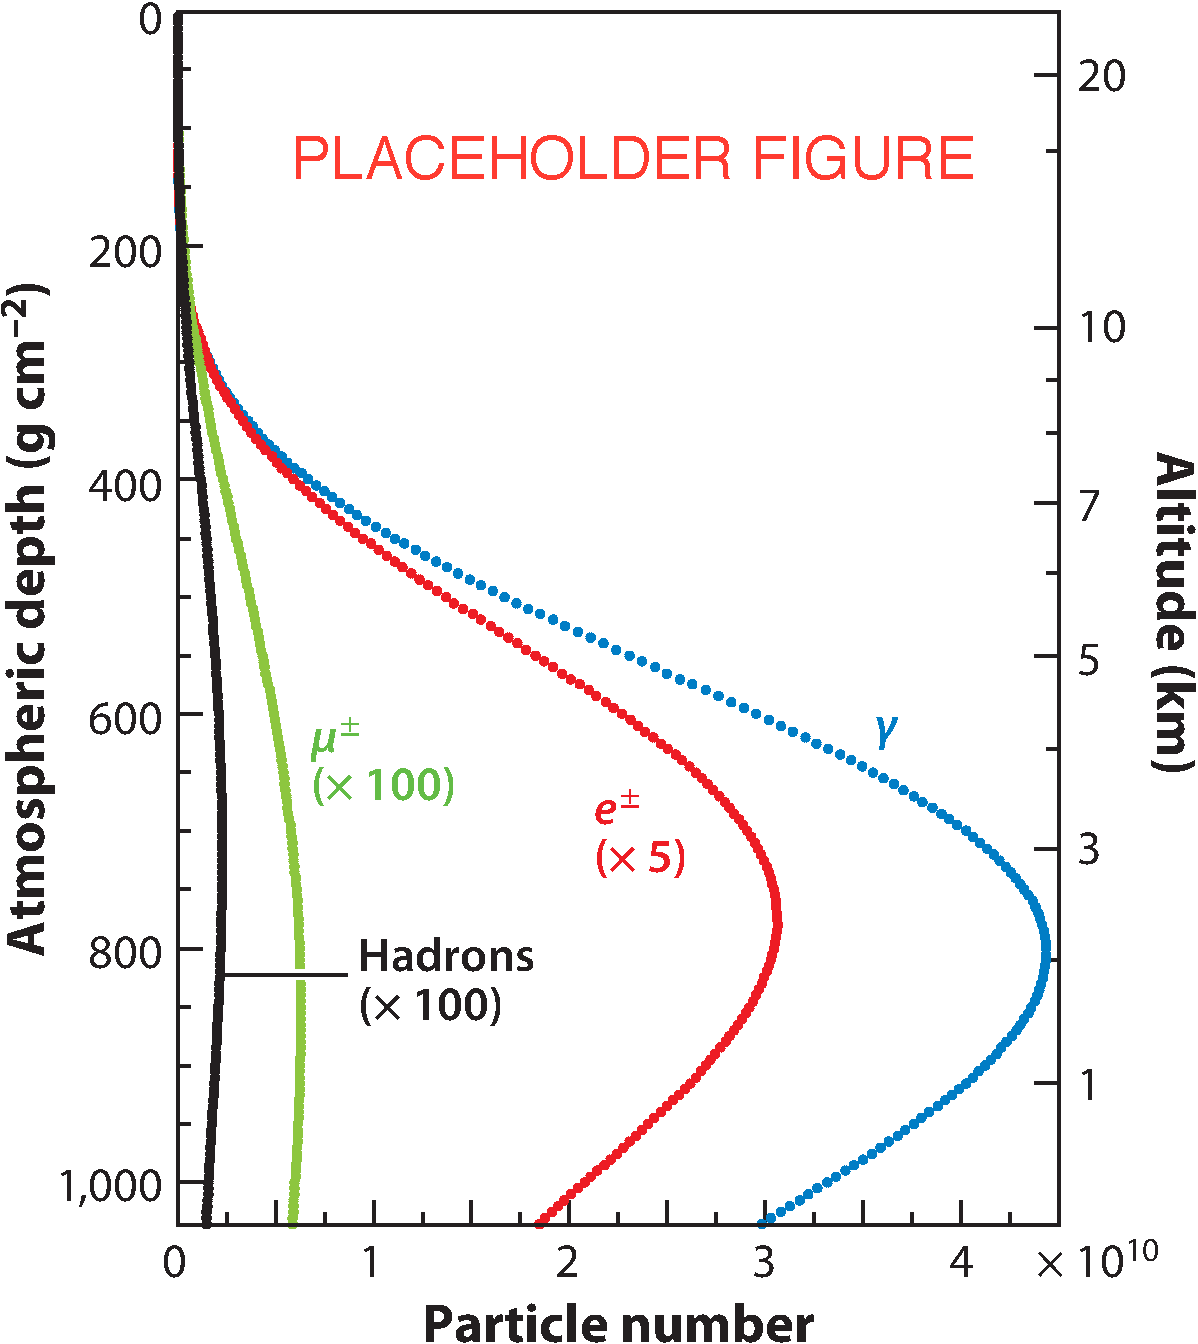
\includegraphics[width=0.6\textwidth]
                    {plots/cosmic-rays/longitudinal_profile}
    \caption{The longitudinal shower profile showing the number of particles in the air shower as a function of the atmospheric depth. Different types of particles are shown separately. The depth at which the maximum number of particles exists is called Xmax. \cite{engel2011eas}}
    \label{fig:longitudinal_profile}
\end{figure}

% The interactions also result in deflections, so the shower expands lateraly.
In the particle interactions and scattering processes the particles emerging from the interaction may have a different direction vector than the incident particle. The transverse momentum of the secondaries mean that the shower extends laterally, away from the shower axis.

% Shower shower profile (CORSIKA).
% Each shower with the same primary energy can develop very differently, chance processes. The size (number of particles) varies for cosmic rays of same energy.
In \cref{fig:shower} all traces of the particles in an air shower are shown. The showers is shown from the side. This is the typical development of a shower. However, the discussed processes are all chance processes. Sometimes the first interaction will be higher, sometimes much later. The multiplicity also differs between collisions of the same energy. The first interactions greatly affect the development of the rest of the shower. In \cref{fig:shower_size_distribution} the total number of leptons reaching ground level (with energy above thresholds) is shown for simulated showers of different energies. All showers are from the zenith. As can be seen the final number of particles varies greatly, spanning about a decade. Showers with a lower point of first interaction will result in larger shower sizes. Note that  here ground level is approximately sea level, at $X = \SI{1080}{\gram\per\centi\meter\square}$, so the shower is past Xmax. If the observation level would be around $X_{max}$ the shower sizes would be more consistent.

\begin{figure}
    \centering
    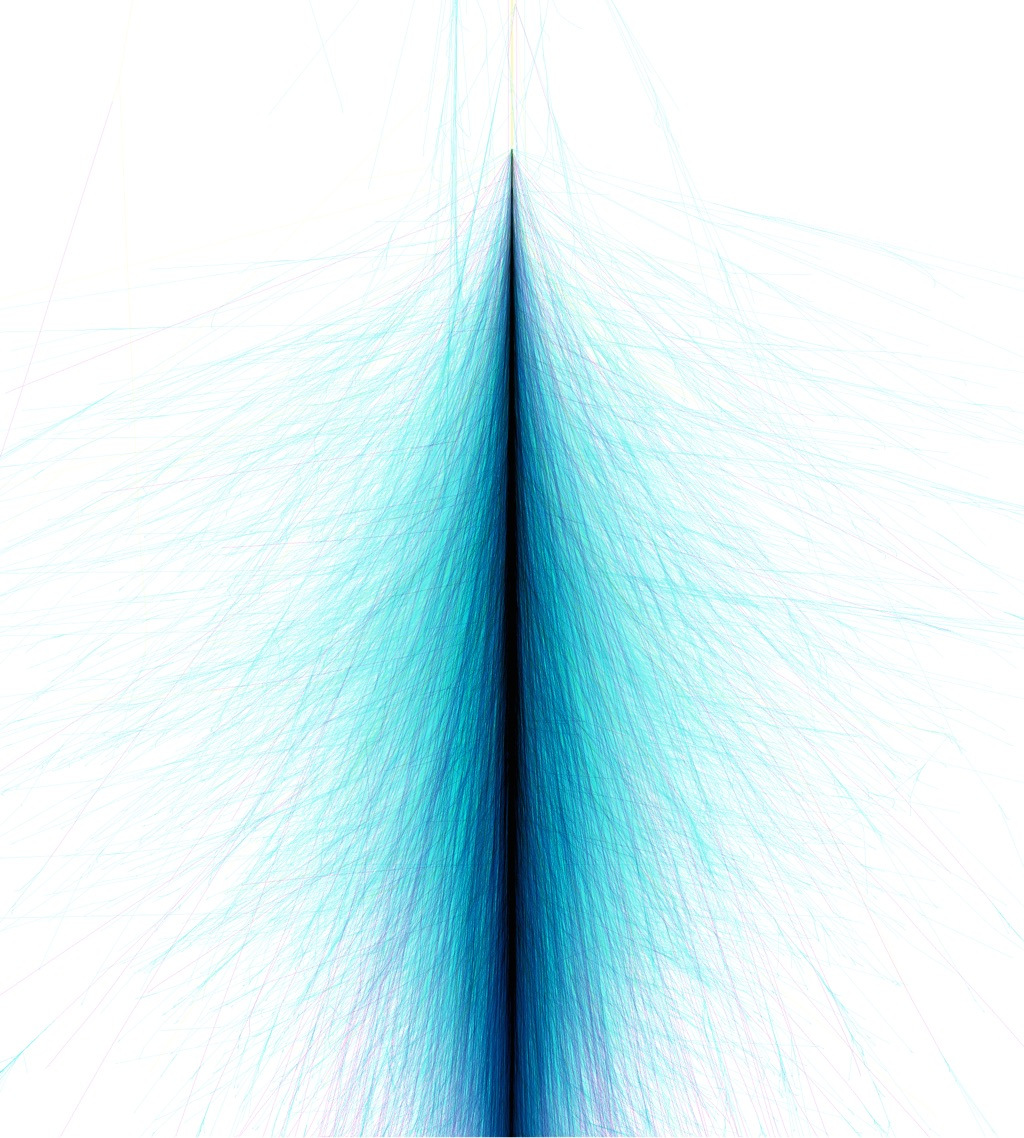
\includegraphics[width=0.6\textwidth]
                    {plots/cosmic-rays/shower.jpg}
    \caption{Particle tracks of a simulated air shower from a proton with $E = \SI{e16}{\eV}$. The different types of particles are shown with different colors. This shows both the longitudinal and lateral distribution of particles. Motion in the y-direction is ignored. \cite{heck2013corsika}}
    \label{fig:shower}
\end{figure}

\begin{figure}
    \centering
    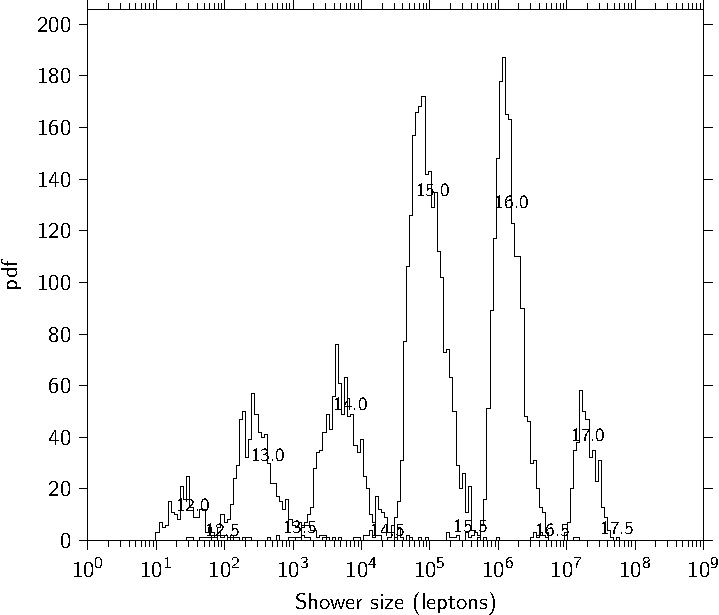
\includegraphics[width=0.6\textwidth]
                    {plots/cosmic-rays/shower_size_distribution}
    \caption{Number of leptons on ground distributions versus the energy of the primary particle. The variation from shower to shower means that showers will have a different number of particles reaching ground level, eventhough the primary energy was equal. The variations can be as high as a factor 10.  \cite{heck2013corsika}}
    \label{fig:shower_size_distribution}
\end{figure}


\section{Shower front}

% What the shower looks like as it reaches ground, how this shape is a result of the various interactions.

Of interest to ground-based experiments is what the observables on the ground are. The focus will be on the leptons and high energy gamma rays which can be efficiently detected. The shower development in the air happens fast, many of the created particles have a lot of energy and move at relativistic speeds. The direction of motion remains approximately equal to the initial incident particle. If a snapshot were made during the development of the shower a 'front' would be seen. This is the shell of particles moving towards ground \cite{drescher2006eas}. The highest density will be at the core of the shower axis, with a lower density towards the edges. The thickness of the front will increase with increasing core distance because of the different path lengths the particles took to get there will vary more. The front of the front is not flat/tangent, at larger core distances the first particles will be delayed relative to the tangent plane of the first particle, again because that particles will have needed to travel a longer distance to get to the sides. Theoretically a causal front exists, a (semi-)sphere with the first interaction at its origin which moves with speed $c$. Since no particle is known to travel faster than light there should be no particle from the shower that reaches ground before the causal front. The expected curvature of the front is approximately a sphere. In \cref{fig:schematic_front} the discussed features are shown in a schematic representation of the front.

The shower front can be defined in multiple ways, either as a snapshot in time or the front as is passes an observation level. In the first case the $z$ (height) coordinates of particles is relavant, in the second it is replaced by the arrival time $t$ of the particles at a certain observation level. Since particle detectors are fixed at a certain altitude the second definition will be used when refering to the shower front.

\begin{figure}
    \centering
    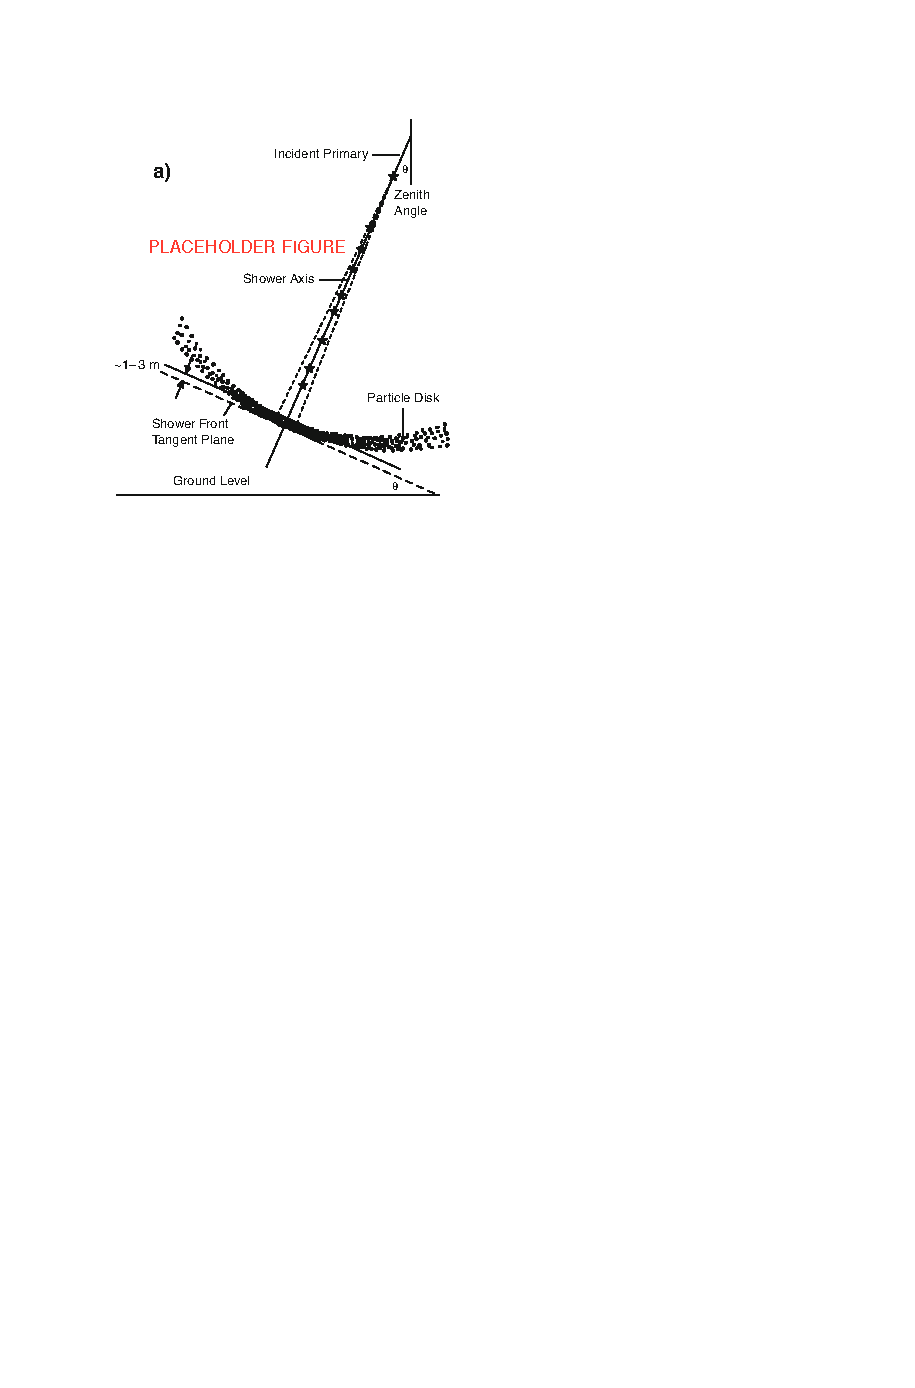
\includegraphics[width=0.6\textwidth]
                    {plots/cosmic-rays/schematic_front}
    \caption{A schematic representation of the front as it approaches ground level. The dots represent shower particles. This is a snapshot in time, all particles are moving with approximately $c$ towards the ground. The particles on the front will reach the ground first followed by those behind. Near the core the density of particles in higher and they are closer to the front. Away from the core the front is curved away from a flat shower front plane. The thickness (rise time) of the front increases with core distance. \cite{grieder2010eas} to \cite{heck2013corsika}}
    \label{fig:schematic_front}
\end{figure}

% The important distributions related to the shower front.
% LDF for various components, and what influences it.
The particle density at the core of the shower front is highest and then quickly deminishes as the distance increases. In \cref{fig:ldf} the typical particle density as a function of core distance is shown for different particle types. The most common particles are high energy (\SI{>3e9}{\eV}) gamma rays, followed by electrons (\SI{>3e9}{\eV}), then muons (\SI{>3e11}{\eV}). The density decreases rapidly with increasing distance. The lateral density distribution can be parameterized by a so called lateral distribution function (LDF). Several such parameterizations exist, the most well known is the Nishimura-Kamata-Greisen (NKG) \cite{apel2006nkg}. This is given by
%
\begin{equation}
    \label{eq:nkg}
    \rho(r) = N_\mathrm{e}\, c(s) \left(\frac{r}{R_0}\right)^{s - 2} \left(1 +
    \frac{r}{R_0}\right)^{s - 4.5},
\end{equation}
%
where $\rho(r)$ is the electron density at a given core distance, $N_e$ the number of electrons at ground level, $R_0$ the Molière radius, $s$ the shower age parameter, and $c(s)$ given by
%
\begin{equation}
    c(s) = \frac{\Gamma(4.5 - s)}{2\pi R_0^2\, \Gamma(s)\,\Gamma(4.5 - 2s)}.
\end{equation}

The NKG was derived analytically for showers initiated by an \Pelectron or \Pphoton. This makes it a bad fit for describing hadron-induced showers. For the \kascade experiment a modified NKG was derived and tested with Monte Carlo data. It was found to fit the simulated data better, espectially at large core distances. The overall particle density increases with the energy of the primary particle.

\begin{figure}
    \centering
    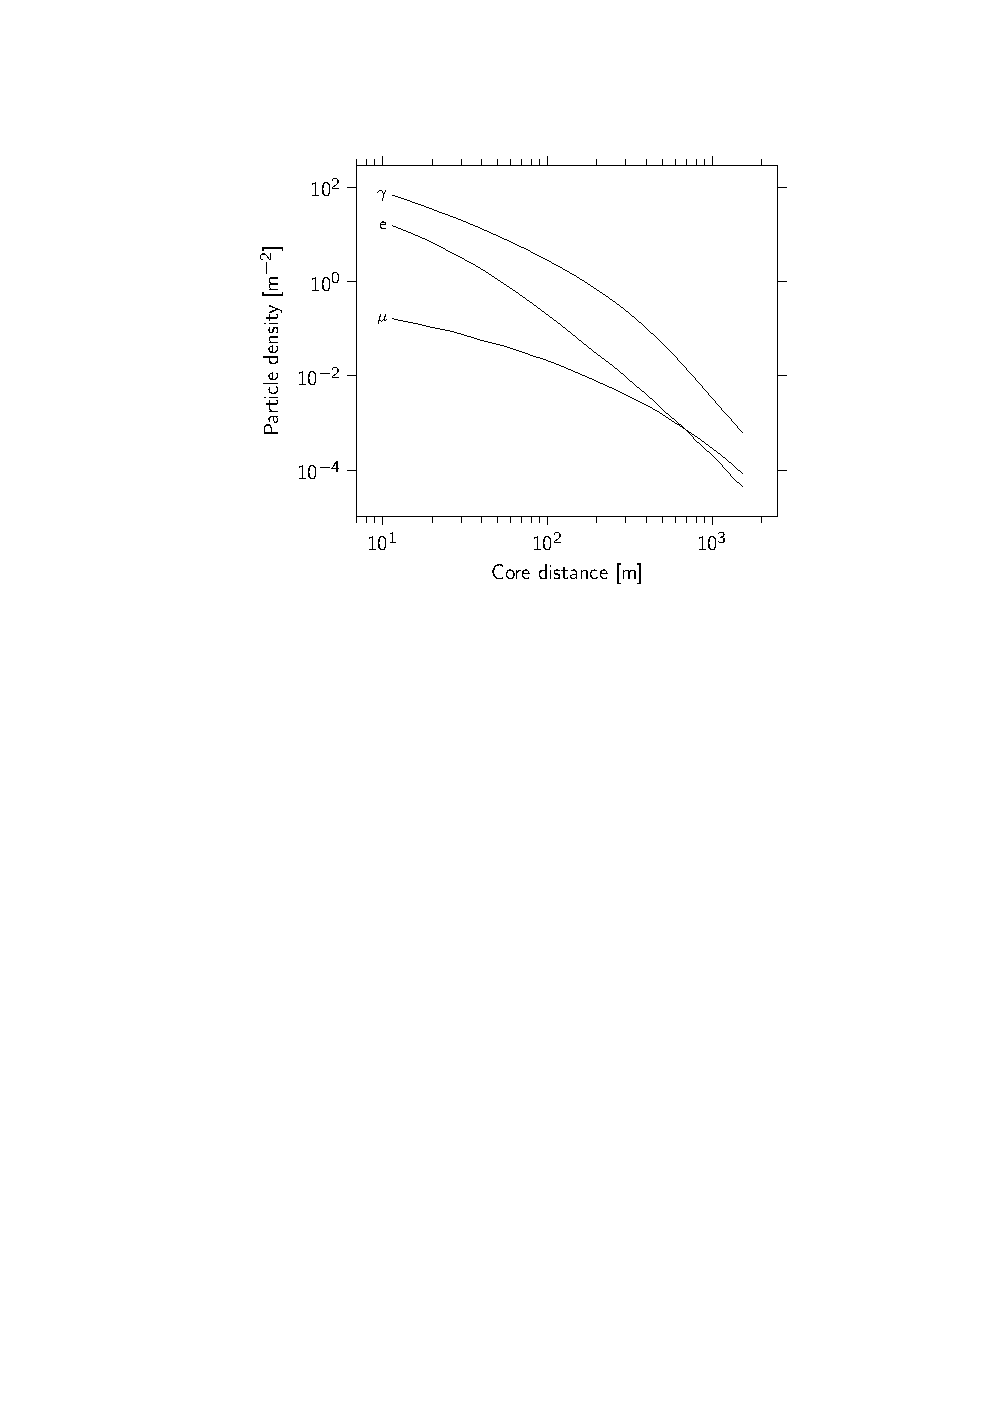
\includegraphics[width=0.6\textwidth]
                    {plots/cosmic-rays/ldf}
    \caption{Lateral density distribution]
The particle density as a function of core distance for a shower of $E = \SI{e16}{\eV}$. The contribution from the different components is shown.}
    \label{fig:ldf}
\end{figure}


\subsection{Temporal shower front}

% At various core distances the temporal profile.
The temporal structure of the shower front can be seen for various core distances in \cref{fig:temporal_profile}. Shortly after the first few particles most of the front crosses the obervation level, followed by a long tail of straggling particles. Further from the core the particle density is lower and the spread in arrival times increases.

A hypothetical particle detector would be able to detect more particles the closer it was to the shower core. The probability is high that one of the detected particles would be close to the front. At larger distances the density becomes lower, so fewer particles will be detected. The chance that one of the detected particles was close to the front decreases. Moreover, the temporal distribution is much wider so the probability that the particles is even further delayed from the front is larger.

\begin{figure}
    \centering
    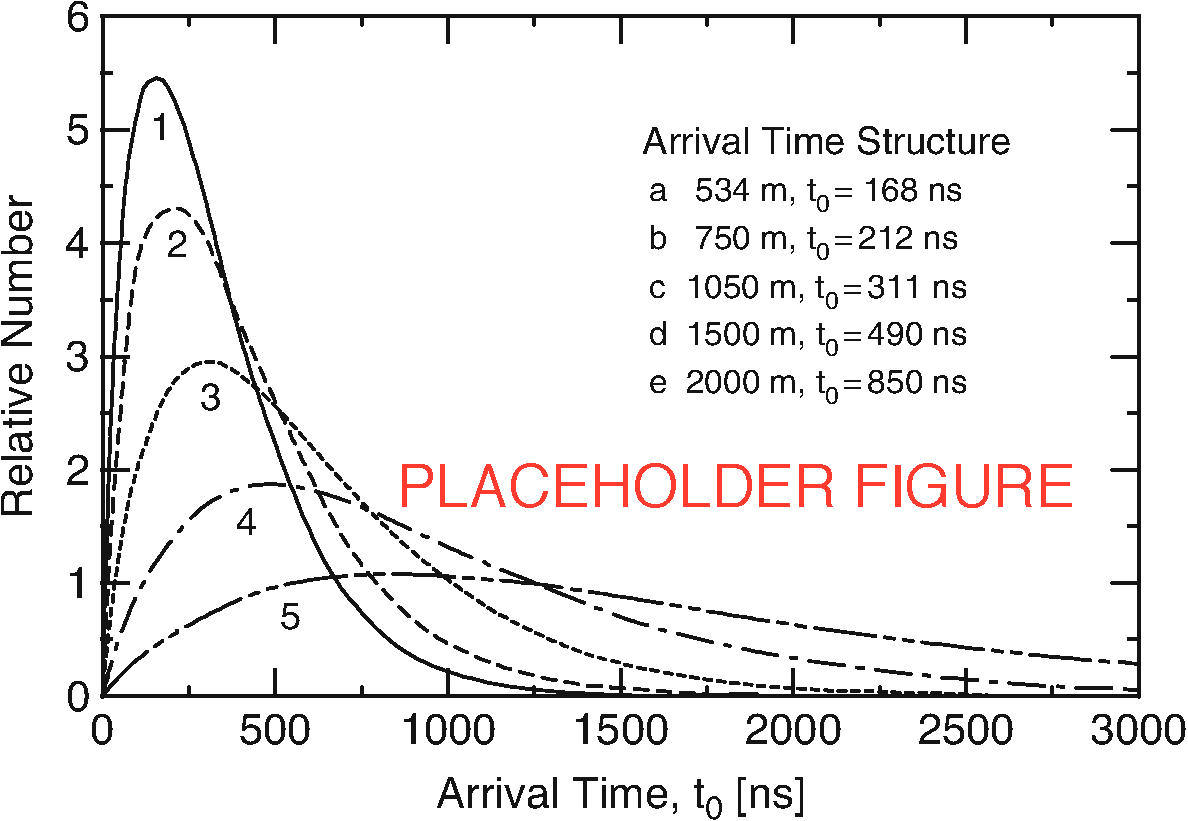
\includegraphics[width=0.6\textwidth]
                    {plots/cosmic-rays/temporal_profile}
    \caption{Temporal structure of shower front, for various core distances]
The temporal structure of the shower front at different core distances for different types of particles. $t = \SI{0}{\ns}$ is the time the first particle reaches ground. Muons arrive first, followed by the gammas and electrons. Each has a long tail of stragglers. \cite{grieder2010eas} to \cite{heck2013corsika}}
    \label{fig:temporal_profile}
\end{figure}


The energy distribution of the leptons in the front is shown in \cref{fig:energy_front}. The cutoff at the left side is due to the cuts in the simulation for electrons at \SI{3e9}{\eV}. It can be seen that the mean particle energy decreases with increasing core distance. Since also the particle density decreases with increasing core distance most of the shower energy content is still close to the core.

\begin{figure}
    \centering
    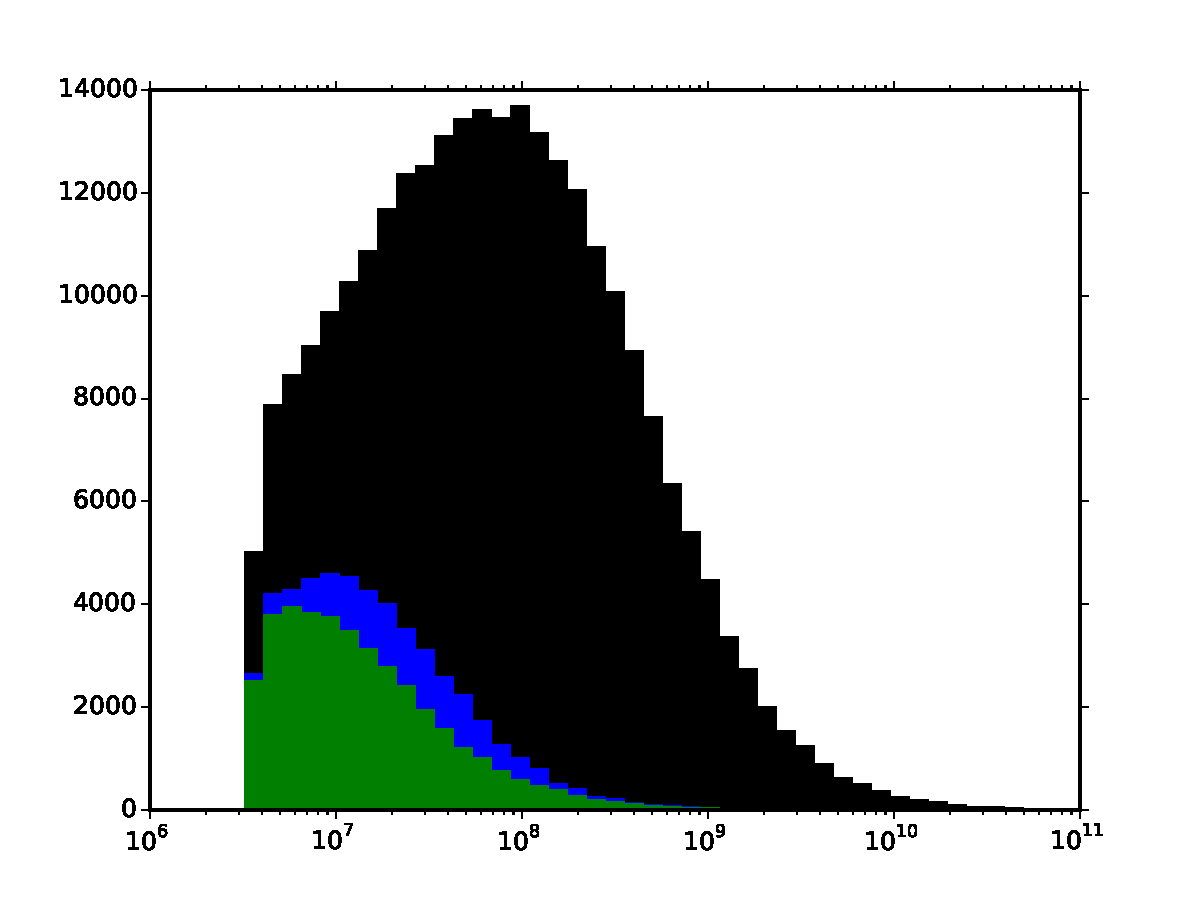
\includegraphics[width=0.6\textwidth]
                    {plots/cosmic-rays/energy_front}
    \caption{Energy distribution of electrons in the shwower front at various core distances. This is for a simulated $E = \SI{e16}{\eV}$ vertical proton shower. The energy distributions are shown for $r$ in \SIrange{0}{10}{\meter} (black), \SIrange{90}{110}{\meter} (blue), and \SIrange{180}{240}{\meter} (green). \cite{heck2013corsika} [todo; axis labels, x: Particle energy, y: Particles]}
    \label{fig:energy_front}
\end{figure}


% Explain why muons are earlier than electron/gamma.
% Explain why the front is curved and the thickness of the front varies.
In \cref{fig:temporal_per_particle} the temporal distribution for the various particle types is shown. The muons are typically first, muons are produced in the charged pion decays and then travel uninterrupted to ground. Electrons and gammas on the other hand undergo many interactions before reaching ground. In each of these interactions there is a possibility of gaining transverse momentum (scattering), this means the trace from the particle on the ground back to the initial interaction will be less of a straight line, more jagged. On average the electrons arrive after the muons.

\begin{figure}
    \centering
    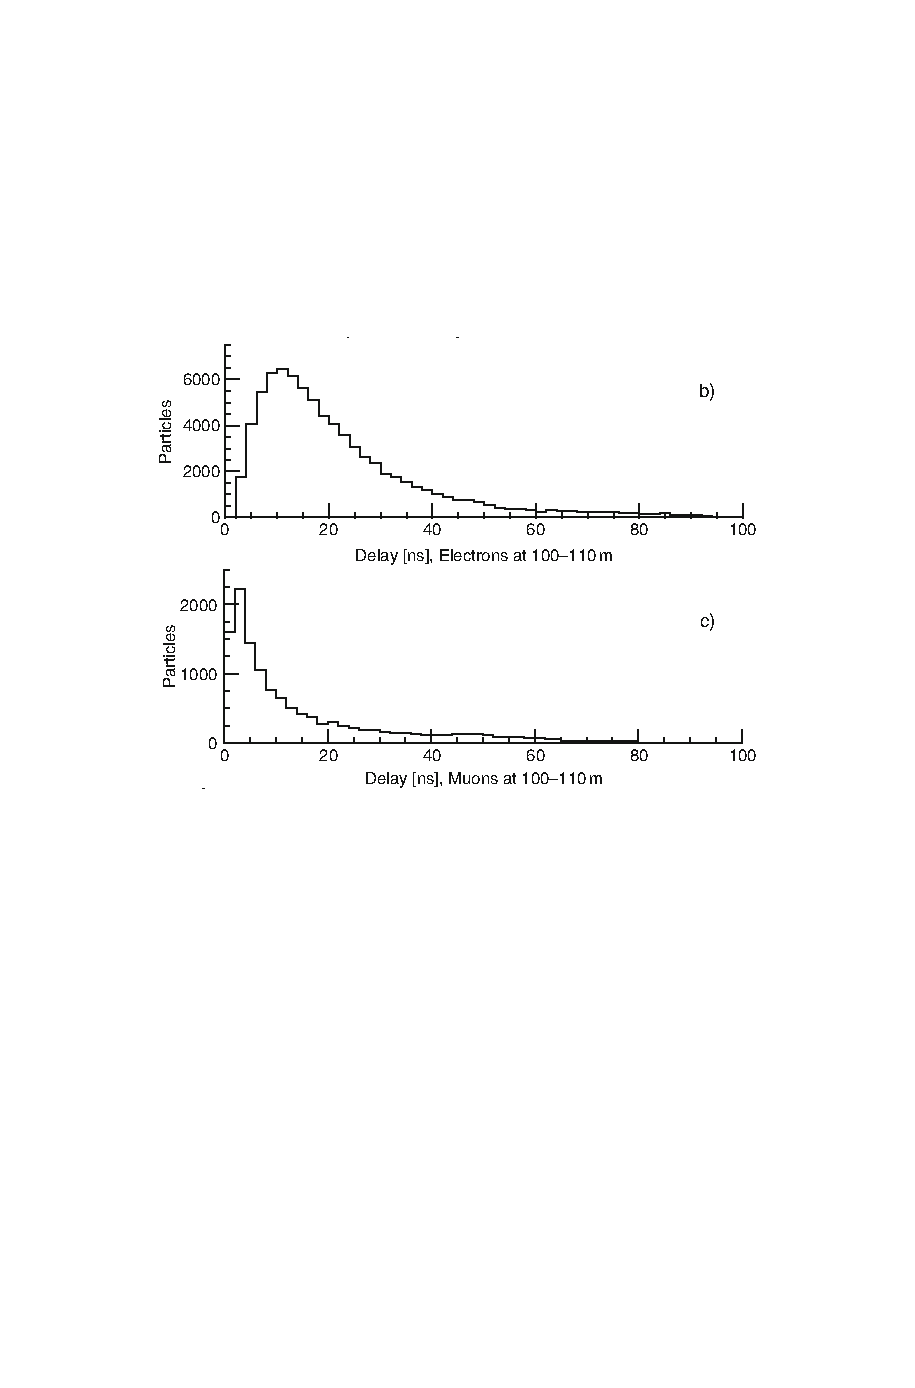
\includegraphics[width=0.6\textwidth]
                    {plots/cosmic-rays/temporal_per_particle}
    \caption{Temporal distribution per particle type. At the same core distance the muons arrive before the electrons and have a sharper distribution. \cite{grieder2010eas}}
    \label{fig:temporal_per_particle}
\end{figure}

%The relation between the curvature/rise time to other shower properties.
%
%
%\begin{figure}
%    \centering
%    \includegraphics[width=0.6\textwidth]
%                    {plots/cosmic-rays/curvature_front}
%    \caption{Mean shower front curvature as a function of the shower size. The interaction altitude of a shower affects the curvature of its shower front. \cite{grieder2010eas}}
%    \label{fig:curvature_front}
%\end{figure}
%
%[Front rise time as function of size (or interaction altitude)]
%The mean shower front rise time at various core distances as a function of the shower size. The combined rise time for muons and electrons is shown.
%

\section{Design criteria}

\subsection{Physics questions}

% Explain why we want to detect cosmic rays; possibly identify sources (anisotropy)
Many unanswered questions remain in cosmic rays research. The main unresolved problem is the origin of cosmic rays. To find out which objects and by which processes are cosmic rays accelerated. This is difficult to determine for low energy charged cosmic rays, because their direction changes so drastically due to magnetic fields. However, direct observations of bremsstrahlung, synchrotron radiation, and neutral pion decay at the sources may reveal their origin, but that is out of the scope of this experiment. High-energy cosmic rays travel in straighter paths and may be used to backtrace to an origin.

% verifying GZ-effect
Composite cosmic rays may undergo spallation due to solar photons. In this process they break into smaller part which may produce simultaneous but geographically separated air showers. This is called the Gerasimova-Zatsepin (GZ) effect. This processes has not yet been conclusively detected. It is a rare process and requires simultaneous detections at very large (\SIrange{1e2}{1e4}{\kilo\meter}) distances, with good direction reconstruction of each shower.

% find features in the shower front, detect jets in air showers, e/mu ratio, temporal/lateral
The full shower development in the atmosphere is not fully understood. The shower front is the result of the interactions in the atmosphere. Understanding of the shower front provides better insight into what interactions happened in the shower development. For instance the existence of jets in the shower. Jets result in irregularities in the shower front at small scales. A fine grid of detectors is required to detect these irregularities. Also the temporal and lateral structure of the shower front require further investigation. By using high sampling frequencies the temporal structure may be unraveled.

% investigate relations to lightning strikes
Theories exists about a possible connection between lightning storms and cosmic rays. When the conditions are right for a lightning storm a cosmic ray air shower may be the initiator. Cosmic rays may help with ionisation of the atmosphere, providing a path for the lightning to strike. [CWI, LOFAR, RU]

\subsection{Educational potential}

% educate high-school students in research and physics.
Finally cosmic rays can be used to educate high school students. Currently subjects like quantum mechanics, relativity, electromagnetic fields, and particle physics are part of the `Nieuwe Natuurkunde' (NiNa) program for physics at high schools  \cite{overheid2012nina}. `Natuur, Leven en Technologie' (NLT) is also a subject for students interested in physics \cite{overheid2011nlt}. It consists of multiple domains from which students can choose, one of these is `Stellaire informatie en processen', which translates to Stellar information and processes. The data analysis also provides practical teaching material for informatics students. Cosmic rays provide an excellent teaching subject for these topics.

\subsection{Detection ...}

% Which cosmic rays do we want to detect, energy range; large area for very energetic cosmic rays, but also detectors close together for efficiently detecting low energy cosmic rays.
In order to efficiently detect high energy cosmic rays a large detection area is required (or a very patient researcher), because of the low flux. Individual detectors need to be spaced such that enough of the shower front is sampled to allow reconstruction of properties of the shower and primary cosmic ray. For low-energy cosmic rays the detectors need to be placed closer in order to sample the shower front. The flux of low energy cosmic rays is much higher, so much less total area is required to in a short time detect a lot of them.

For low energy showers the density drops off to rapidly and direction reconstruction will be hard when detectors are to close and the time resolution can not keep the angular resolution high. The energy range of interest is from \SI{e14}{\eV} and up. The upper limit will be determined by the final size and duration of the project.

\begin{figure}
    \centering
    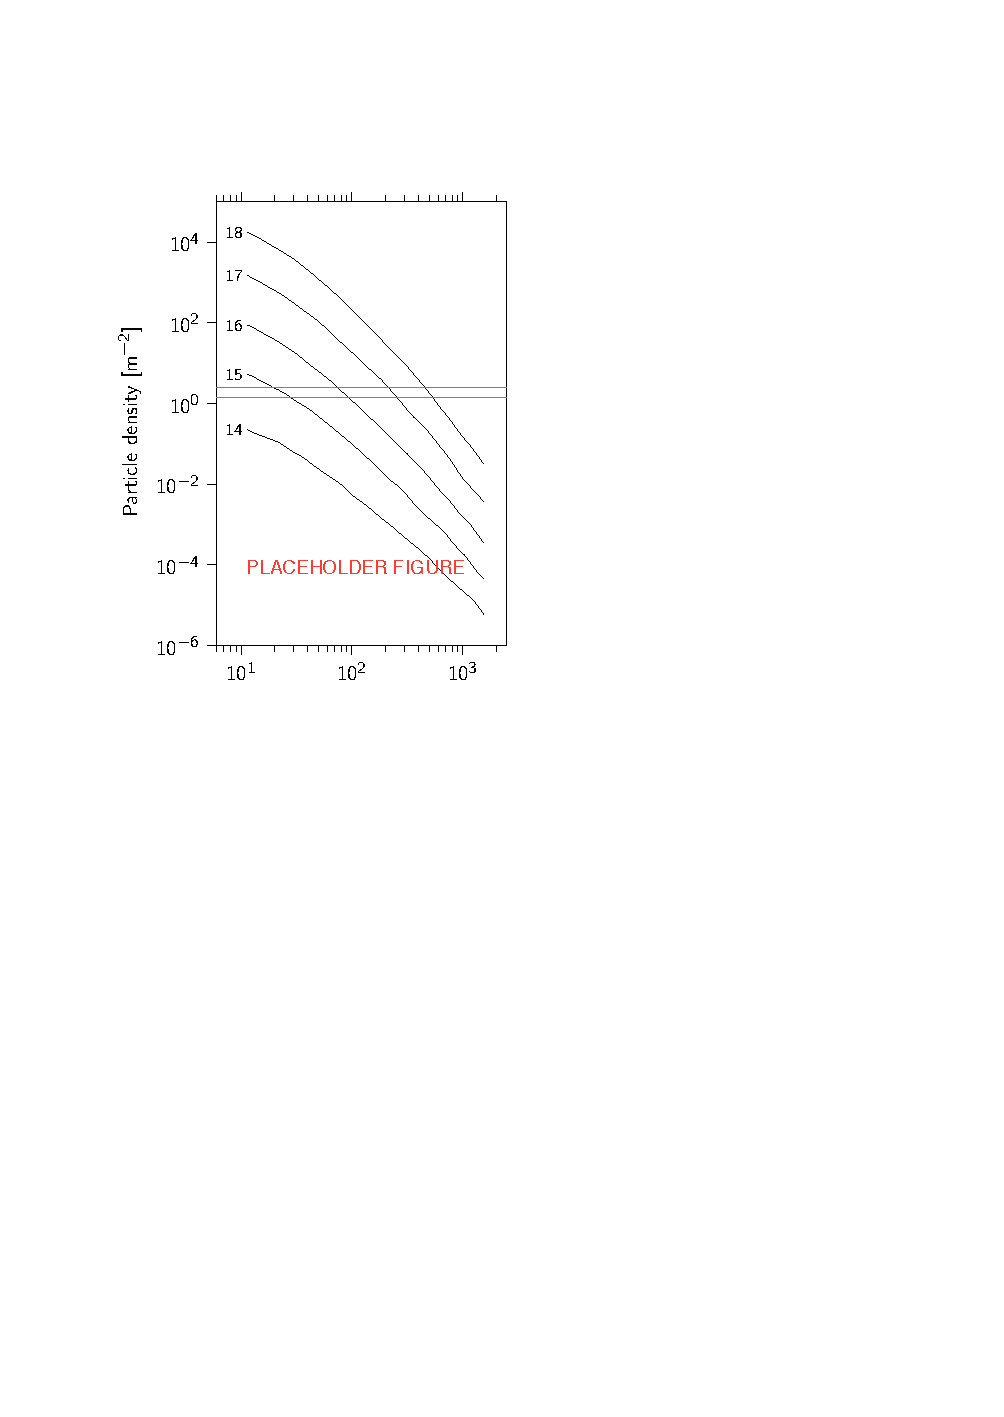
\includegraphics[width=0.5\textwidth]
                    {plots/cosmic-rays/ldf_energies}
    \caption{LDF for E = \SIrange{e14}{e20}{\eV} showers (e + mu). This gives the limits of detecting showers, depending on core distance and detector size. (do not show horizontal lines)}
    \label{fig:ldf_energies}
\end{figure}

% What do we want to determine for each air shower; time of arrival, direction of the shower axis, position of the core, and energy of the primary.
% Which properties of the shower need to be measured to determine this
By detecting the arrival time of particles from the same shower at various locations the shower front is sampled. This allows for the reconstruction of the shower. Using the arrival times the direction of the shower can be reconstructed. Using the density the core position and energy can be obtained. These reconstructions are not independent, knowledge about the core position improves direction reconstruction, and vice-versa shower axis direction makes the estimation of expected particle densities more accurate.

% What are the possibilities of identifying a source
The experiment will be based in the Netherlands, with possible extensions to other countries. From the Netherlands the Northern sky is observed. This provides a similar field of view to the TA and \kascade experiments, which are at latitudes \SI{39.3}{\degree} and \SI{49.1}{\degree}. \nikhef is at latitude \SI{52.3}{\degree}. The visible-sky map, assuming a zenith acceptance of \SI{60}{\degree}, in equatorial coordinates is shown in \cref{fig:visible_sky_map}. The anisotropy measurement of cosmic rays at very high energies is difficult to achieve due to the low flux. The Auger and TA experiments have only a handful of detections above \SI{e20}{\eV}. These experiments have exposures of \SI{7250}{\kilo\meter\squared\year\steradian} (TA) and \SI{48029}{\kilo\meter\squared\year\steradian} (Auger), which is a meaure of their area, angular acceptance, and run time \cite{abbasi2015combined}. Measurement of the isotropy at lower energies is important for verification of the expectation.

\begin{figure}
    \centering
    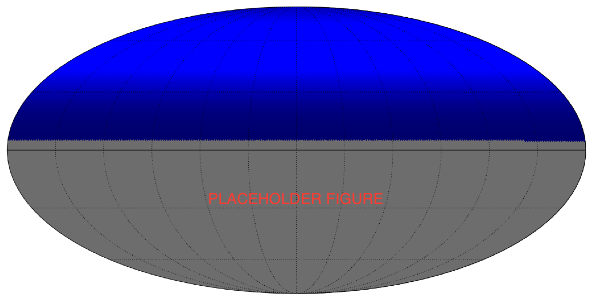
\includegraphics[width=0.6\textwidth]
                    {plots/cosmic-rays/visible_sky_map}
    \caption{Equatorial sky map (mollweide) highlighting part of universe which is above the horizon in the Netherlands. Similar field of view to TA/KASCADE.}
    \label{fig:visible_sky_map}
\end{figure}


\section{Design for detection}

% Detector the particles in the shower front, not the fluorescence/Cherenkov. For several reasons; particle detectors are much cheaper, provides higher uptime. Also detect extensive air showers during day time, moon nights, and with other sources of light pollution.
In \cref{sec:other_observables} methods other than particles detectors for the observation of air showers were mentioned. These will not be considered, as these methods are much more expensive and have lower duty cycles. For experiments such as TA and Auger they do provide excellent independent calibration of the surface particle detectors and extra information about the shower. This experiment will use particle detectors for the detection of cosmic rays.

% What properties/observables of the air shower particles need to be measured.
%  - Arrival time of the particles (leptons) and their number.
%  - Accurate arrival time is needed for direction (using shower front shape).
The arrival time of particles and number of particles in a detector can be used to reconstruct the shower. The accuracy with which this can to be measured depend on the properties of the shower and detectors. For increasing distance between detectors a lower arrival time accuracy is required to achieve the same direction reconstruction accuracy. With increasing core distance the particle density decreases, while the rise time of the shower front increases. This makes it more likely that fewer particles are detected and that those that are detected are further delayed from the causal front. This increases the uncertainty in direction reconstruction.

\subsection{Detection probability}
\label{ssec:detection_probability}

%  - Accurate particle count is needed for energy/core (using lateral density).
Important to consider is the likelihood of actually detecting a shower. For a given charged particle density $\rho$ and a detector with area $A$ the probability of detecting exactly $k$ particles is given by the Poisson distribution. Here $\lambda$ is the expected number of particles, i.e. $\lambda = \rho A$ and $P_k$ the probability.
%
\begin{equation}
    \label{eq:poisson}
    P_k(\lambda) = \frac{\lambda^k \mathrm{e}^{-\lambda}}{k!} \ .
\end{equation}
%
This assumes the detectors are \SI{100}{\percent} efficient at detecting charged particles. The important probability is the probability of not detecting any particle (i.e. $k = 0$) given a particle density, given by
%
\begin{equation}
    P_0(\lambda) = \mathrm{e}^{-\lambda} \ .
\end{equation}
%
Which gives the probability of detecting at least one particle via
%
\begin{equation}
    P_p(\lambda) = 1-P_0(\lambda) \ .
\end{equation}

% Each particle detector will have a background from low energy showers, such showers are very abundant, but only few particles (mainly muons) reach ground level.
Not all detected particles will be desired. A big component of the background comes from low energy showers (\SI{<e14}{\eV}) which produce only a couple muons at sea level, and even fewer electrons. Such low energy cosmic rays are very abundant. Instead of resulting in an instantaneous high density of particles these showers produce a random background of particles. These showers produce to few particles to effectively sample the shower front. In \cref{fig:particle_density} the total particle flux at various atmospheric depths is shown. At sea level the muon flux dominates. The high muon flux relative to electrons is dominated by low energy showers. For higher energy showers (\SI{>e13}{\eV} for vertical showers) the electron-muon ratio favors the electrons.

\begin{figure}
    \centering
    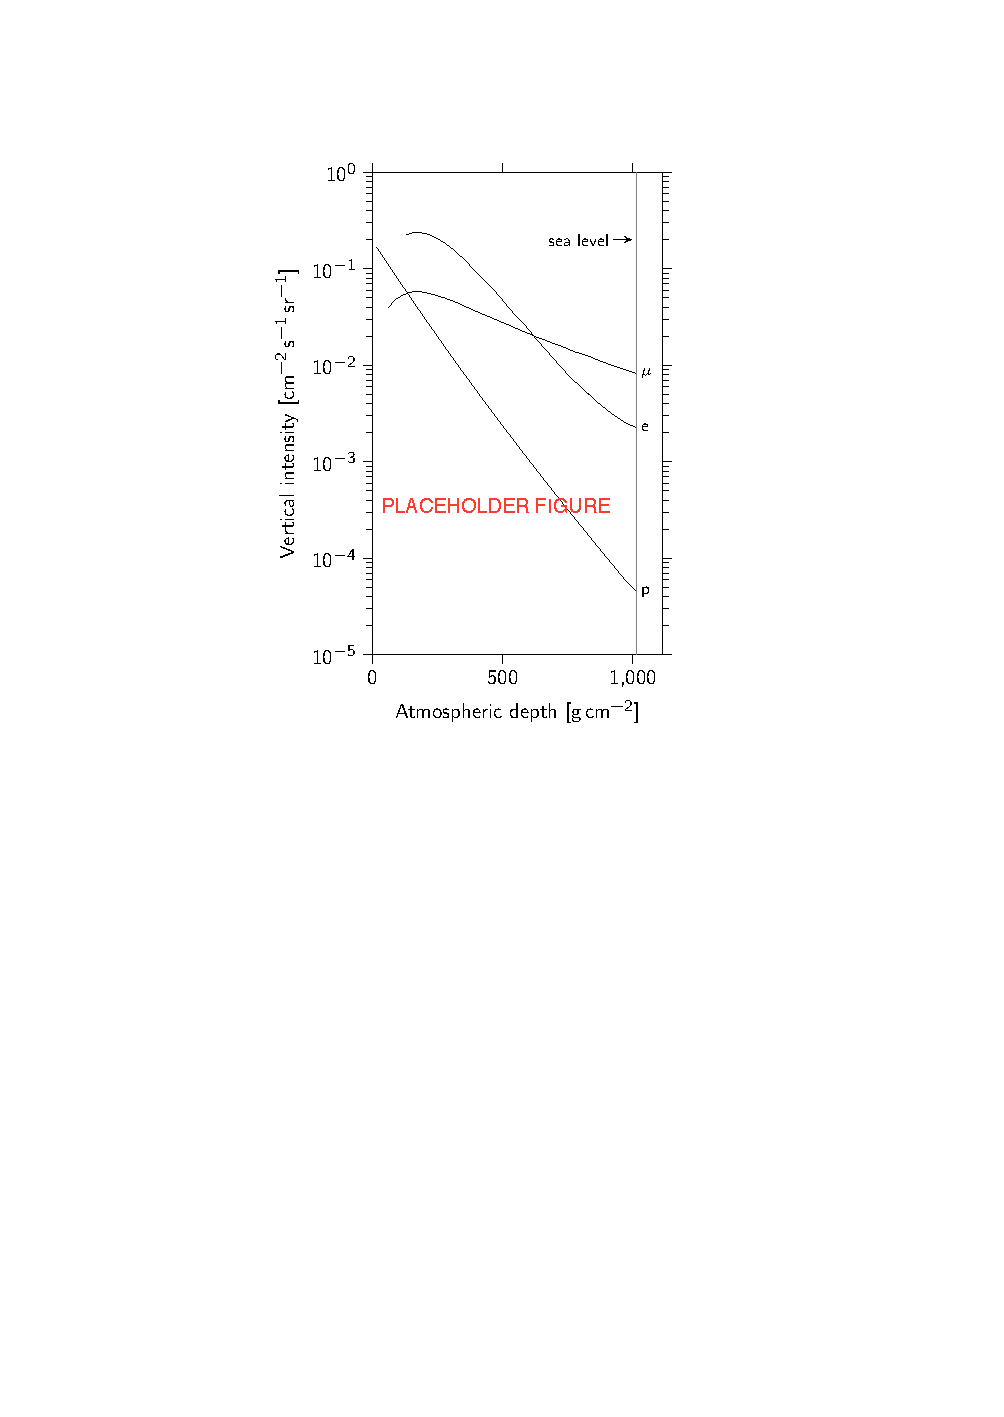
\includegraphics[width=0.5\textwidth]
                    {plots/cosmic-rays/particle_density}
    \caption{Particle flux composition as function of atmospheric depth, to show the flux of particles at ground level, todo: filter for only particles with 'enough' energy (like Grupen fig7.10)}
    \label{fig:particle_density}
\end{figure}

% How to filter the background away by using a coincidence trigger. Two (or more) simultaneous, unrelated, detections in separated detectors is unlikely.
The particles from individual showers are correlated in time in contrast to the random background. These showers can be distinguished from the background by looking for time-correlated particles. This might be possible with a single detector which looks for short bursts of many particles. However, this does not provide data for reconstruction, since the arrival time and density is only known at one position. Multiple combined detectors using a time-correlated trigger is more sensitive to lower particle densities, since only one particle needs to be detected per detector. Moreover, it provides data for reconstruction. Using two detectors to distinguish the particles from the background by requiring at least one particle in each detector makes the probability of detection $P_2(\lambda) = P_p^2(\lambda)$, assuming the particle density is equal at both detectors. The size of and distance between the detectors will determine the lower energy limit.

% How to figure out where should the detectors be placed (relative to each other)
%  - For low energy (\SIrange{e14}{e15}{\eV}) showers the detectors need to be closely spaced (\SI{10}{\meter}) otherwise the density in the detectors becomes to low to effectively detect them.
%  - For high energy (\SIrange{e18}{e20}{\eV}) showers the detectors need to be placed further apart (\SI{>500}{\meter}) otherwise the area covered by the detectors is to small and only few high energy showers will be detected.
The efficiency with which two detectors can detector a shower can be estimated. Assume that the shower core is precisely between the two detectors. In such a case the detection efficiency is highest. If the shower was closer to either detector the probability of detection for one detector would go up, but it falls for the other detector, reducing the overall probability. Using an estimate of the particle density for (vertical) showers as described in \cref{eq:nkg} the probability of detection can be estimated for showers of different energies depending on the size of the detectors and the distance between the detectors.

The relation between the median shower size (number of electrons at sea level) and primary energy (see \cref{fig:shower_size_distribution}) can be approximated by the following relation
%
\begin{equation}
    N_{\Pe} = 10^{\log\left(\frac{E}{\si{\eV}}\right) - 10.2} \ ,
\end{equation}
%
which is valid for (semi-)vertical showers. As the zenith angle of showers increases above \SI{15}{\degree} the shower size noticeably decreases. Also the energy at which the transition from mostly muons to mostly electrons at ground is at higher values for larger zenith angles. A better fit may be achieved by adding an extra parameter
%
\begin{equation}
    N = 10^{\log\left(\frac{E}{\si{\eV}}\right)^y - x} \ .
\end{equation}
%
This can be fitted more accurately to the median electron, muon and total lepton sizes (per zenith angle). For the number of electrons the values $x = 13.3$ and $y = 1.07$ best describe results from simulated air showers (protons from the Zenith).

$P_2$ is a function of $P_0$, which can be written as a function of the shower energy, core distance, and detector size as follows
%
\begin{equation}
    P_0(E, r, A) = \mathrm{e}^{-A\rho(N_{\Pe}(E), r)} \\ .
\end{equation}
%
With this the expected detector efficiency for a detector setup can be estimated for various shower energies. Inclined showers can also be investigated, in case of a flat detector the effective detection area is smaller by $\cos \theta$. The particle density is harder to estimate because different parts of the shower have different path lengths through the atmosphere. This makes the particle density distribution ellipse shaped. Also the effective distance between a detector and the shower core changes depending on the azimuthal angle of the shower.

% Why are for reconstruction multiple detection points needed.
To be able to fully reconstruct the direction of an air shower at least three detection points are required. Having two detection points with arrival times provides a constraint on the shower axis, but a plane of possibilities remain \cite{schultheiss2016pair}, a third detection point (not on the same line) constrains the shower axis. This can either be achieved by a single station with three or more detectors (short distances), or by combining detections from multiple stations (larger distances). Using a 3-detector station the probability of detecting at least one particle in each is given by $P_p^3(\lambda)$. If the station had even more detectors ($n$) but still required at least 3 in coincidence the probability of detection becomes
%
\begin{equation}
    P_{\mathrm{min}=3}(\lambda) = \sum_{k=3}^{n} \binom{n}{k} P_p^k P_0^{n-k} \ .
\end{equation}

\subsection{Background rate}

% Depending on size of coincidence window how much background remains. Reconstruction should identify bad/accidental events.
Consider the 2-detector setup again in which both need to detect a particle within a short time window to make certain both are from the same shower. The rate of muons at ground level is approximately $f_{\Pmump} = \SI{~200}{\Pmump\per\meter\squared\per\second}$. Most should have entirely uncorrelated arrival times. Since the distribution is random some might arrive simultaneously. The expected rate of random coincidences can be calculated by
%
\begin{equation}
    \label{eq:background_rate}
    R_{\mathrm{background}} = 2 \tau A^2 f^2 \ ,
\end{equation}
%
where $\tau$ is the time window, $A$ the detector area, and $f$ the background flux. $2 \tau A f$ gives the total time window which is considered. Note that \cref{eq:background_rate} is only applicable if $\tau < (A f)^{-1}$ and $R_{\mathrm{background}} \ll Af$.

The time window should be at least the distance between the two detectors divided by the light speed. That should be the most extreme case for a shower to arrive horizontally in line with the detectors. Longer time differences are possible due to different transport time in the detector and the rise time and curvature of the shower front.

\subsection{Practical considerations}

% The detectors need to be reliable to prevent continuous maintenance tasks, and to last the length of the experiment, MoU expects ~5 years.
Ideally the detectors operate without maintenance. The components might have finite lifetimes or require recalibration after some time. If many detectors require frequent service and maintenance this will cost time that could otherwise be spent on data analysis. Basically the costs of the experiment go up. Using tried-and-tests components that have been shown to be reliable for long periods are preferred.

% Cost effective detectors so high-schools can participate in the project
Making detectors larger makes them more likely to detect particles. The downside is that the detector becomes less easy to handle, more expensive, efficiency uniformity may worsen, and saturation might occur sooner. A good balance needs to be determined.

% The detector needs to be safe to handle by students
% Detectors need to be durable so they can survive the typical Dutch weather
The experiment is meant to be accessible for high schools, the detectors need to be fairly easy to handle. If the detectors would be placed inside schools it may be difficult to find a safe location and the roof material might affect the detections. In order to have enough space to place the detectors the most obvious location would be on the roof. If the detectors are outside proper protection from weather effects need to be considered.
